\documentclass[12pt]{book}
%Gummi|065|=)
\title{\textbf{Pathfinding su giochi grid-based}}
\author{Lentisco Francesco\\
N86001092}
\date{}
\usepackage{graphicx}
\usepackage[linesnumbered,algoruled,boxed,lined]{algorithm2e}
\usepackage{float}
\usepackage{fancyvrb}
\usepackage{cprotect}
\usepackage{listings}
\usepackage{color}
\usepackage{amsfonts}
% or
\usepackage{amssymb}
\usepackage{tikz}
\usepackage{amsmath}
\usepackage{subcaption}
\usepackage{setspace}
\begin{document}
\onehalfspacing
\maketitle

\SetKwProg{Fn}{Function}{}{}

\chapter{Introduzione}
\section{Problematica del pathfinding}
\par{Il requisito base di ogni agent di un videogioco \`e essere in grado di muoversi all'interno dell'ambiente di gioco. Il problema del movimento nei videogiochi si pu\`o scomporre in due sottoproblemi: locomozione e \emph{pathfinding}. La locomozione si occupa dello spostamento fisico di un agente di gioco mentre il pathfinding si occupa di pianificare un percorso valido verso la nuova posizione desiderata dall'agente di gioco.}
\par{Tuttavia il problema del pathfinding non riguarda solamente i videogiochi. Esso \`e infatti ampiamente discusso anche in ambito di networking e robotica. L'approccio al pathfinding \`e fondamentalmente simile nei diversi campi di ricerca, ma i requisiti e i vincoli possono invece differire notevolmente. I videogiochi essendo per loro natura dei sistemi real-time e multiagent impongono dei vincoli molto stretti al problema del pathfinding. Altri fattori come la dinamicit\`a dei moderni videogiochi aumentano ulteriormente il grado di complessit\`a del problema. L'obiettivo di questa tesi \`e dunque fornire una visione di insieme sul problema del pathfinding riguardo i videogiochi, ponendo l'attenzione su diverse tecniche di ricerca su grafi, i loro vantaggi e criticit\`a accennando anche ad alcuni aspetti riguardanti il \emph{game design}.}

\section{Grafi di navigazione}
\par{Affinch\`e un algoritmo di pathfinding possa effettuare una ricerca in un ambiente di gioco, deve anzitutto essere in grado di \emph{comprendere} quest'ultimo. La geometria dell'ambiente di gioco pu\`o essere molto complessa e irregolare e pertanto inadatta per effettuarvi ricerche. Occorre dunque che l'ambiente di gioco sia semplificato separatamente in una \emph{mappa di navigazione} fruibile agli algoritmi di ricerca.}
\par{La struttura dati pi\`u semplice in grado di rappresentare la mappa di navigazione di un ambiente di gioco \`e il grafo. Si definisce grafo come una coppia $G = (V, E)$ di insiemi finiti con V insieme dei nodi ed E insieme degli archi, tali che gli elementi di E siano coppie di elementi di V ($E \subseteq V\times V$). Un vertice (o \emph{nodo}) \`e semplicemente il dato che vogliamo rappresentare come grafo, mentre un arco \`e un collegamento tra due vertici. Ogni vertice pu\`o avere molteplici archi che lo collegano ad altri vertici del grafo.}
\par{Un grafo che contiene i dati di navigazione di un ambiente di videogioco \`e chiamato \emph{grafo di navigazione} (\emph{navgraph}). In un grafo di navigazione, ogni nodo rappresenta una possibile locazione dell'ambiente di gioco. Inoltre ogni nodo mantiene una lista di nodi direttamente accessibili da quel nodo (nodi adiacenti) con relativo costo di attraversamento (peso di un arco).}
\begin{figure}[htp]
\centering
\includegraphics[scale=0.30]{/home/notsaved/Documenti/graph.jpg}
\caption{grafo pesato}
\label{graph}
\end{figure}

\par{Un grafo di navigazione pu\`o essere consiederato come una \emph{astrazione} dell'ambiente di gioco. Il metodo di astrazione comporter\`a la grandezza e la complessit\`a del grafo di navigazione risultante. Vedremo nelle prossime sezioni alcuni comuni tecniche.}

\subsection{Waypoint}
\par{I waypoint sono una comune tecnica di astrazione per creare un grafo di navigazione dell'ambiente di gioco. Tipicamente, si posizionano manualmente dei punti di navigazione (che rappresentano i nodi del grafo risultante) nell'ambiente di gioco durante la fase di design del livello. Questi vengono poi collegati manualmente o automaticamente (collegando i nodi che hanno tra loro una linea di visibilit\`a diretta).}
\par{La figura \ref{waypoint1} mostra il posizionamento e il collegamento di waypoint in un ambiente di gioco di esempio. Come possiamo osservare, tale tecnica minimizza i numeri di nodi necessari, ma ci\`o comporta che il grafo risultante potrebbe non coprire la totalit\`a delle possibili locazioni dell'area di gioco.}
\begin{figure}[htp]
\centering
\includegraphics[scale=0.50]{/home/notsaved/Downloads/waypoint1.png}
\caption{grafo di navigazione basato su waypoint creato manualmente}
\label{waypoint1}
\end{figure}
\par{Esistono inoltre tecniche di generazione di waypoint automatizzate, ma a causa del loro grado di complessit\`a il loro utilizzo \`e limitato tipicamente ad una fase di preprocessamento del livello. Purtroppo tali tecniche, oltre a non poter garantire una copertura della totalit\`a dell'area di gioco, possono includere nodi ed archi ridondanti, influendo negativamente sulle prestazioni degli algoritmi di ricerca.}
\par{Una delle varianti \`e basata sulle linee di visibilit\`a. I nodi generati vengono posizionati automaticamente sugli spigoli dei poligoni convessi ed infine connessi tra loro a due a due se esiste una linea di visibilit\`a diretta. Tuttavia questo approccio, come possiamo vedere in figura \ref{waypoint2}, comporta un notevole numero di nodi e archi ridondanti.}
\begin{figure}[htp]
\centering
\includegraphics[scale=0.50]{/home/notsaved/waypoint2.png}
\caption{grafo di navigazione basato su waypoint creato automaticamente con approccio di linee di visibilit\`a}
\label{waypoint2}
\end{figure}
\par{In generale, un altro problema di cui questa tecnica soffre \`e la dinamicit\`a dell'area di gioco. Nel caso in cui avvenga un cambiamento nell'area di gioco non \`e garantita la qualit\`a dei waypoint automaticamente generati, pertanto tale tecnica dovrebbe essere limitata ad ambienti di gioco statici.}
\subsection{Navmesh}
\par{Le navmesh consistono nel rappresentare l'ambiente di gioco utilizzando dei poligoni convessi. In questo caso un poligono rappresenta una intera area nell'ambiente di gioco, invece che una singola locazione. Ogni singola area \`e connessa alle aree adiacenti.}
\par{Esistono diverse metodologie di suddivisione dello spazio di gioco, accomunate dal fatto che le forme utilizzate devono essere convesse poich\`e non deve esserci alcuna ostruzione tra due punti all'interno dello stesso poligono. Un tipico esempio \`e la suddivisione dell'ambiente di gioco in triangoli mediante Triangolazione di Delaunay dalla quale \`e possibile ottenere una ulteriore suddivisione in poligoni di Voronoi .} 
\begin{figure}[htp]
\minipage{0.42\textwidth}
  \includegraphics[width=\linewidth]{/home/notsaved/Documenti/Delaunay.png}
  \caption{Triangolazione di Delaunay con tutti i circumcerchi e i loro centri (rosso)}\label{fig:awesome_image2}
\endminipage\hfill
\minipage{0.42\textwidth}%
  \includegraphics[width=\linewidth]{/home/notsaved/Documenti/Voronoi.png}
  \caption{Collegando i centri dei circumcerchi si ottiene un diagramma di Voronoi (rosso)}\label{fig:awesome_image3}
\endminipage
\end{figure}
\par{La triangolazione di Delaunay per un gruppo di punti P su un piano \`e un particolare tipo di triangolazione DT(P) tale che nessun punto appartenente a P sia all'interno del circumcerchio di ogni triangolo in DT(P). Come si vede dalla figura \ref{fig:awesome_image2}, si tracciano dei cerchi che connettono i tre vertici di ogni triangolo (circumcerchi) e tali che nessun vertice si trovi all'interno di tali circonferenze. Quando si connettono i centri dei circumcerchi si ottiene un diagramma di Voronoi (Figura \ref{fig:awesome_image3}).}
\par{Dato un insieme finito di punti S, il diagramma di Voronoi per S \`e la partizione del piano che associa una regione V(p) ad ogni punto $p \in S$ in modo tale che tutti i punti del perimetro di V(p) siano pi\`u vicini a p che ad ogni altro punto in S. Tale schema di partizionamento \`e a sua volta utile per estrarre lo scheletro topologico di un'area (voronoi skeleton) che si pu\`o definire come una versione dimagrita di quella forma che \`e equidistante dai suoi confini.}
\begin{figure}[htp]
\centering
\includegraphics[scale=0.60]{/home/notsaved/Documenti/Skel.png}
\caption{scheletro topologico della forma della lettera B}
\label{voronoiskel}
\end{figure}
\par{In generale non ci sono particolari limiti o vincoli sullo schema di partizionamento o sui tipi di poligoni da utilizzare, a patto che le aree generate siano convesse. Le sottoaree generate vengono infine connesse alle sottoaree adiacenti. Anche per le connessioni delle sottoaree esistono molteplici approcci. Uno di questi \`e calcolare il centroide del poligono, ossia, la posizione media di tutti i suoi punti (Figura \ref{fig:centroide}) e connetterlo con il centroide delle aree che condividono un lato. \`E anche possibile utilizzare gli spigoli (Figura \ref{fig:spigoli}), il punto medio dei lati dei poligoni (Figura \ref{fig:punto_medio}), o ancora, utilizzare approcci ibridi (Figura \ref{fig:ibrido}).}

\begin{figure}[htp]
\minipage{0.42\textwidth}
  \includegraphics[width=\linewidth]{/home/notsaved/Documenti/navmesh1.png}
  \caption{mesh collegate mediante il centroide dei poligoni}\label{fig:centroide}
\endminipage\hfill
\minipage{0.42\textwidth}
  \includegraphics[width=\linewidth]{/home/notsaved/Documenti/navmesh2.png}
  \caption{mesh collegate mediante gli spigoli de poligoni}\label{fig:spigoli}
\endminipage\hfill
\minipage{0.42\textwidth}
  \includegraphics[width=\linewidth]{/home/notsaved/Documenti/navmesh4.png}
  \caption{mesh collegate attraverso il punto medio dei lati dei poligoni}\label{fig:punto_medio}
\endminipage\hfill
\minipage{0.42\textwidth}%
  \includegraphics[width=\linewidth]{/home/notsaved/Documenti/navmesh3.png}
  \caption{mesh collegate ibridamente attraverso spigoli e punti medi dei lati dei poligoni}\label{fig:ibrido}
\endminipage
\end{figure}
\par{\`E evidente come i grafi risultanti dalle mesh di navigazione offrano una rappresentazione maggiormente accurata di ambienti complessi rispetto ai waypoints. Tuttavia l'operazione iniziale di suddivisione pu\`o presentare elevati costi computazionali e pertanto tali operazioni vengono tipicamente eseguite offline. }

\subsection{Griglie}\label{subs:griglie}
\par{Utilizzare un array bidimensionale \`e un approccio molto semplice alla rappresentazione di un ambiente di gioco. Ogni elemento dell'array \`e detto \emph{tile} e assume un numero fissato di valori (\emph{tileset}). Per semplicit\`a si assume che gli unici due valori possibili siano bloccato o traversabile.}
\par{Tale approccio vincola dunque l'area di gioco in una matrice con dimensioni fissate di locazioni quadrate che simulano una veduta dall'alto di una regione bidimensionale. 
 Nel progetto proposto ci si \`e serviti di questo approccio per generare delle mappe in modo casuale.}
 \par{Ogni \emph{tile} traversabile dell'area di gioco viene mappato in un nodo nel grafo corrispondente. Un nodo, che corrisponde ad una locazione traversabile \`e connesso a tutti i nodi associati ai tile adiacenti e traversabili. I pesi degli archi che corrispondono a spostamenti ortogonali hanno costo unitario mentre gli archi tra due nodi collegati diagonalmente hanno un costo pari a $\sqrt{2}$.} 
 \begin{figure}[htp]

\minipage{0.32\textwidth}
  \includegraphics[width=\linewidth]{/home/notsaved/Downloads/tile1(1).png}
  \caption{In questa griglia i tile sono connessi ortogonalmente con costo unitario}\label{fig:tile}
\endminipage\hfill
\minipage{0.32\textwidth}%
  \includegraphics[width=\linewidth]{/home/notsaved/Downloads/tile2(1).png}
  \caption{Questa griglia consente spostamenti diagonali con costo di $\sqrt2$}\label{fig:octile}
\endminipage
\end{figure}
 \par{Per riferirsi a un nodo del grafo partendo dalle sue coordinate sulla grigla e viceversa si usano le usuali formule di conversioni:
date le coordinate geometriche x e y di una locazione, il nodo corrispondente avr\`a come identificativo \begin{equation} nodo = y*\mbox{MAP\_WIDTH} + x \end{equation} dove per \emph{MAP\_WIDTH} si intende la larghezza della mappa. Per riottenere invece le coordinate geometriche di un nodo si utilizzano le seguenti formule: \begin{equation} x = nodo \% \mbox{MAP\_WIDTH} \end{equation} \begin{equation} y = nodo / \mbox{MAP\_WIDTH} \end{equation} 
}
\iffalse
\section{Cenni architetturali}

\begin{figure}[htp]
\centering
\includegraphics[scale=0.50]{/home/notsaved/Downloads/gameloop(2).png}
\caption{flowchart generalizzato di un game engine}
\label{gameloop}
\end{figure} \fi
\chapter{Algoritmi di pathfinding}
\par{Il \emph{path-planning} \`e un componente fondamentale della maggior parte dei videogiochi.
Gli \emph{agent} spesso si muovono nell'area di gioco. A volte questo movimento \`e predeterminato dagli sviluppatori del gioco, come ad esempio il percorso di pattugliamento di un area che una guardia deve seguire. I percorsi predeterminati sono semplici da implementare, ma per loro natura sono facilmente prevedibili. Agent pi\`u complessi non sanno in anticipo dove dovranno muoversi. Una unit\`a in un gioco di strategia potrebbe ricevere in tempo reale l'ordine dal giocatore di muoversi in qualsiasi punto sulla mappa, oppure, in un gioco \emph{tile-based} pu\`o succedere che un agent debba inseguire il giocatore nell'area di gioco.
Per ognuna di queste situazioni, l'IA deve essere in grado di computare un percorso adeguato attraverso l'area di gioco per arrivare a destinazione, partendo dalla posizione attuale dell'agent. Inoltre vorremmo che il percorso trovato sia il pi\`u breve possibile.}
\par{La maggior parte dei giochi usa delle soluzioni di pathfinding basate sull'algoritmo chiamato A*. Nonostante sia molto semplice da implementare ed efficiente, A* non opera in genere sulla geometria della mappa di gioco. Esso richiede che tale mappa sia rappresentata in una particolare struttura dati: un grafo pesato e non-negativo.
In questo capitolo verranno presentati gli algoritmi realizzati nel progetto, tra cui Dijkstra, A* e diverse sue varianti.}

\section{Dijkstra}
\label{sec:dijkstra}
\par{Prima di entrare nel vivo degli algoritmi di pathfinding occorre fare alcune precisazioni su cosa si intende per \emph{problema dei cammini minimi}. Nella  teoria  dei  grafi, per shortest-path si intende il cammino minimo tra due vertici, ossia quel percorso che collega due vertici dati e che minimizza la somma dei costi associati all'attraversamento di ciascun arco. Formalmente, }
\par{Sia $G = (V, E)$ un un grafo orientato con funzione di costo $\omega: E \rightarrow \mathbb{R}$ che associa ogni arco ad un valore nell'insieme dei reali. Sia $p=\langle v_0, v_1, ..., v_k \rangle$ un cammino che collega il vertice $v_1$ e al vertice $v_k$, allora il costo di $p$ \`e la somma dei pesi degli archi che lo costituiscono: $$\omega^*(p) = \sum \limits_{i=1}^k \omega(v_{i-1}, v_i) $$.
Dato un cammino $p$ da $v_0$ a $v_k$, $p$ \`e \emph{minimo} sse non esiste un altro cammino $p'$ da $v_0$ a $v_k$ tale che $w^*(p') < w^*(p)$.}
\par{Esistono dunque due varianti del problema: il problema del \emph{cammino minimo} tra una coppia di vertici, e il \emph{problema dei cammini minimi} da un vertice sorgente verso tutti gli altri vertici raggiungibili dalla sorgente. Chiaramente il primo \`e un sottocaso del secondo. }
\par{
L'algoritmo di Dijkstra \`e un algoritmo che risolve il \emph{problema dei cammini minimi} (o Shortest Paths, SP) in un grafo con o senza ordinamento e con pesi non negativi sugli archi.}
\par{Mentre nei videogiochi usualmente si computa il percorso minimo da un punto di partenza a un punto di arrivo, l'algoritmo di Dijkstra \`e realizzato in modo da trovare il percorso pi\`u breve da un punto di partenza verso tutti i restanti punti raggiungibili.
La soluzione includer\`a ovviamente anche l'eventuale punto di arrivo, ma ci\`o comporter\`a in ogni caso uno spreco di risorse computazionali se siamo interessati a un solo punto di arrivo.
Tuttavia pu\`o essere modificato in modo da generare solo il percorso nel quale si \`e interessati, ma sar\`a ancora inefficiente come algoritmo di pathfinding.
}
\par{
Dijkstra \`e un algoritmo iterativo. Ad ogni iterazione, considera un nodo nel grafo ed esamina i suoi archi uscenti (nella prima iterazione considera il nodo di partenza). Ci riferiremo per semplicit\`a al nodo considerato ad ogni iterazione come \emph{nodo corrente}.
Per ogni arco uscente dal nodo corrente, viene esaminato ogni suo nodo terminale $v$ e si memorizza il costo totale del cammino totale percorso fino ad arrivare ad esso (\emph{cost-so-far)} e l'arco dal quale si \`e arrivati ad esso in apposite strutture dati ($dist[v]$ e $prev[v]$ nello pseudocodice). Dopo la prima iterazione, il costo totale del cammino per il nodo terminale di ogni connessione del nodo corrente, \`e uguale alla somma del costo totale del nodo corrente e del peso della connessione verso il nodo terminale.
}
\par{
L'algoritmo tiene traccia dei nodi da visitare in una coda di priorit\`a. La priorit\`a viene stabilita sulla base del costo totale del cammino associato a quel nodo. Nella prima iterazione la coda conterr\`a solo il nodo di partenza con costo totale uguale a 0. Nelle successive iterazioni l'algoritmo estrae dalla coda il nodo con il minor costo totale. Questo sar\`a processato come \emph{nodo corrente}.
}
\par{
Ogni volta che viene esaminato un nodo terminale, l'algoritmo confronta il suo costo totale attuale (all'inizio tutti i nodi vengono inizializzati, assegnandoli un valore di costo di default pari a \emph{infinito}) con quello appena calcolato. Se il costo totale appena calcolato \`e minore di quello precedentemente assegnato a quel nodo terminale, tale valore viene aggiornato. Ovviamente oltre al valore di costo totale viene aggiornato anche il suo predecessore, che diventer\`a l'arco che connette il nodo corrente a quello terminale in esame. Quando si verifica questa condizione significa che l'algoritmo ha trovato un percorso migliore verso quel nodo terminale.
}
\par{
L'implementazione canonica di Dijkstra termina quando la coda \`e vuota, ossia, quando tutti i nodi appartenenti al grafo sono stati visitati e processati. Tuttavia per risolvere un problema di pathfinding, l'algoritmo pu\`o terminare prima che tutti i nodi vengano processati, ossia, quando il nodo di arrivo \`e il nodo con la priorit\`a pi\`u bassa nella in coda.
}
\par{
Una volta raggiunto il nodo di arrivo, viene estratto il cammino percorrendo a ritroso tutte le connessioni usate per arrivare a quel nodo fino a raggiungere il nodo di partenza.
}

\scalebox{0.75}{
\begin{minipage}{\linewidth}
\begin{algorithm}[H]
\PrintSemicolon
\caption{Dijkstra Shortest Path}
  \LinesNumbered
%This is to hide Begin keyword
 \Fn{DijkstraShortestPath((V,E), source)}{
 	\tcc{array per tenere traccia del costo totale del percorso fino a quel nodo}
 	$dist[source] \longleftarrow 0 $\; 
 	\tcc{coda di priorit\`a}
 	 $Q \longleftarrow \emptyset$\;
 	\ForEach{$v \in V$ }{
		\If{v $\neq$ source}{
		 	 $dist[v] \longleftarrow \infty$\;
		 	 $prev[v] \longleftarrow \emptyset$\;
		}
		$Q.\textbf{add}(v, dist[v])$\;
 	}
	\While{$Q \neq \emptyset$}{
		$u \longleftarrow Q.\textbf{extractMin}()$\;
		\ForEach{$v \in V | \exists (u,v) \in E$}{
			$alt \longleftarrow dist[u] + \textbf{lenght}(u,v)$\;
			\If{alt \textless dist[v]}{
					 	 $dist[v] \longleftarrow alt$\;
					 	 $prev[v] \longleftarrow u$\;
					 	 $Q.\textbf{updatePriority}(v,alt)$\;
			}
		}
	}
 } 
\end{algorithm}
\end{minipage}
}

\par{
Tenendo presente che la coda di priorit\`a \`e implementata come uno \emph{heap di Fibonacci} e che la complessit\`a delle operazioni di \textbf{extractMin}() e \textbf{updatePriority}() sono rispettivamente $\mathcal{O}(log(n))$ e $\Theta(1)$, la complessit\`a dell'algoritmo nel caso peggiore \`e di $\mathcal{O}(|E| + |V| \log|V|)$.
}
\section{A*}
\label{sec:astar}
La maggior parte dei sistemi di \emph{pathfinding} odierni sono basati su questo algoritmo, data la sua efficienza, semplicit\`a di implementazione e ampi margini di ottimizzazione.
Diversamente dall'algoritmo di Dijkstra, A* \`e pensato per la ricerca del percorso minimo \emph{point-to-point}.
\par{
Il funzionamento dell'algoritmo \`e molto simile a quello di Dijkstra. A differenza di quest'ultimo, che sceglie sempre prima il nodo con il minor \emph{cost-so-far}, A* sceglier\`a il nodo candidato che \emph{pi\`u probabilmente} porter\`a al percorso pi\`u breve. Per far ci\`o, A* utilizza delle funzioni \emph{euristiche}. Maggiore sar\`a l'accuratezza della funzione euristica utilizzata, tanto pi\`u l'algoritmo sar\`a efficiente.
}
\par{
A* funziona iterativamente: in ogni iterazione considera un nodo del grafo ed esamina i suoi archi uscenti. Il nodo corrente viene scelto usando un criterio di selezione simile a quello di Dijkstra, ma con la significativa differenza dell'euristica.
}
\par{
Come Dijkstra, per ogni arco uscente dal nodo corrente, A* esamina il suo nodo terminale $x$ e memorizza il costo totale del cammino percorso fino ad arrivare ad uno di essi (\emph{cost-so-far)} e l'arco dal quale si \`e arrivati. Inoltre A* memorizza un valore in pi\`u, ovvero, una stima del costo totale $f(x)$ del percorso dal nodo di partenza al nodo di arrivo attraverso $x$. Questa stima \`e data dalla somma di due valori: il costo totale \emph{reale} dal nodo sorgente fino al nodo $x$ (\emph{cost-so-far} al quale ci riferiremo come \emph{g(x)}) e la distanza (euristica) dal nodo $x$ fino al nodo di arrivo a cui ci riferiremo come \emph{h(x)}.
}
\par{
Pertanto \emph{f(x) = g(x) + h(x)}. Come vedremo, \emph{f(x)} fornisce la chiave dell'ordinamento della coda di priorit\`a dell'algoritmo}.

\par{
A* tiene traccia dei nodi scoperti ma ancora da processare in una coda, a cui ci riferiremo come \emph{Open}, e dei nodi gi\`a processati in una lista \emph{Closed}. I nodi saranno inseriti nella coda \emph{Open} appena saranno scoperti lungo gli archi uscenti dal nodo corrente. Essi verranno successivamente trasferiti nella lista \emph{Closed} una volta che diventeranno essi stessi nodo corrente.
}
\par{Diversamente da Dijkstra, viene estratto dalla coda \emph{Open} il nodo con il minor valore \emph{f(x)}. In tal modo si processeranno per primi i nodi pi\`u promettenti.}
\par{Potrebbe accadere che si arrivi ad esaminare un nodo appartenente alla coda \emph{Open} o alla lista \emph{Closed} e si debbano modificare i suoi valori di costo. In questo caso ricalcoleremo il valore di \emph{g(x)} come al solito e se esso \`e minore di quello gi\`a memorizzato, allora verr\`a aggiornato.}
\par{Diversamente da Dijkstra, A* pu\`o trovare cammini migliori per nodi che sono gi\`a stati processati, e che quindi si trovano nella lista \emph{Closed}. In particolare, nel caso in cui durante una ricerca si incontra un nodo $x$ appartenente alla lista \emph{Closed} si valuta se il valore \emph{g(x)} \`e maggiore del costo del percorso appena scoperto vuol dire che abbiamo scoperto un percorso migliore, e dovremmo aggiornare il predecessore di $x$ e il valore \emph{g(x)}. Tuttavia quando un nodo viene messo nella lista \emph{Closed}, vuol dire che tutti i suoi archi uscenti sono stati processati. Pertanto aggiornare i valori del nodo $x$ non sar\`a sufficiente, giacch\`e la modifica deve essere propagata lungo tutte le sue connessioni uscenti.}
\par{Esiste un approccio molto semplice per ricalcolare e propagare i valori aggiornati di un nodo appartenente alla lista \emph{Closed}, ossia estrarlo dalla lista \emph{Closed} e inserirlo nuovamente nella coda \emph{Open} con i suoi valori aggiornati. Esso stazioner\`a nella coda finch\`e non verr\`a estratto e processato nuovamente. In tal modo le sue connessioni potranno a loro volta aggiornate nuovamente.}
\par{In molte implementazioni dell'algoritmo, A* viene fatto terminare quando il nodo di arrivo \`e il nodo con la minima priorit\`a nella coda \emph{Open}. Tuttavia come abbiamo visto, un nodo con il minor costo potrebbe essere rivisitato in un secondo momento. Non possiamo pi\`u garantire pertanto che il nodo minimo nella coda \emph{Open} sia quello che porti ad un cammino minimo. Di qui, la maggior parte delle implementazioni di A* possono produrre risultati non ottimali. Altre implementazioni terminano non appena il nodo di arrivo viene visitato non aspettando che esso diventi il pi\`u piccolo nodo nella coda \emph{Open}. In ogni caso si ammette che il risultato finale potrebbe essere non ottimale, pertanto sar\`a a discrezione dello sviluppatore scegliere l'opportuna terminazione.}
\SetKwRepeat{Do}{do}{while}%

\scalebox{1}{
\begin{minipage}{\linewidth}

\begin{algorithm}[H]
\PrintSemicolon
\caption{A* Shortest Path}
  \LinesNumbered
  \KwIn{Graph (V,E), Node source, Node target}
%This is to hide Begin keyword
 \Fn{AStarShortestPath((V, E), source, target)}{
	$\textbf{g}(source) \longleftarrow 0$\;
	$\textbf{parent}(source) \longleftarrow source$\;
 	 $Open \longleftarrow \emptyset$\;
 	 $Closed \longleftarrow \emptyset$\;
 	 $Open.\textbf{Insert}(source, \textbf{g}(source) + \textbf{h}(source))$\;

	\Do{$Open \neq \emptyset$}{
		$u \longleftarrow Open.\textbf{extractMin}()$\;
		\If{$u = target$}{\tcc{check whether we reached the target vertex}\Return{"path found}"}
		\tcc{We haven't reached the target vertex yet; expand the node}
		$\textbf{expandNode}((V, E), u)$\;
		$Closed.\textbf{add}(u)$\;

	}\Return{"no path found"}
 }
\end{algorithm}
\end{minipage}
}

\scalebox{1}{
\begin{minipage}{\linewidth}
\begin{algorithm}[H]
\PrintSemicolon
\setcounter{AlgoLine}{15}
\caption{Expand Node}
 \Fn{expandNode((V, E), u)}{
 		\ForEach{$v \in V | \exists (u,v) \in E$}{
			$tentativeGScore \longleftarrow \textbf{g}(u) + \textbf{c}(u,v)$\;
			$fScore \longleftarrow tentativeGScore + \textbf{h}(v)$\;
			\If{$v \in Closed \lor v \in Open$}{\tcc{We re-encountered a vertex. It's either in the open or closed list.}
				\If{$tentativeGScore \geq \textbf{g}(v)$}{\tcc{Ignore path since it is non-improving}
					$continue$\;
				}
				$\textbf{g}(v) \longleftarrow tentativeGScore$\;
				$\textbf{parent}(v) \longleftarrow u$\;
			\If{$v \in Closed$}{
			\tcc{it's in the closed list. Move node back to open list, since we discovered a shorter path to this node}
				$Closed.\textbf{remove}(v)$\;
				$Open.\textbf{insert}(v, fScore)$\;
			}\Else{\tcc{It's in the Open list}
			$Open.\textbf{updatePriority}(v,fScore)$\;
			}
		}\Else{\tcc{We discovered a new node}
		$\textbf{g}(v) \longleftarrow tentativeGScore$\;
		$\textbf{parent}(v) \longleftarrow u$\;
		$Open.\textbf{Insert}(v, fScore)$\;
		}
		}}
\end{algorithm}
\end{minipage}
}

\par{Esattamente come per Dijkstra, si recupera il cammino compiuto percorrendo ricorsivamente tutte le connessioni accumulate dal nodo di arrivo fino a quello di partenza.}
\par{Generalmente la parte euristica dell'algoritmo viene implementata come una funzione.
Di seguito riporteremo alcune delle pi\`u comuni funzioni euristiche.
 Siano $u$ e $v$ due nodi con coordinate rispettivamente di $(x_1, y_1)$ e $(x_2, y_2)$ }
\begin{itemize}
\item Manhattan distance: $H(u,v) = |x_1 - x_2| + |y_1 - y_2|$
\item Euclidean distance: $H(u,v) = \sqrt{(x_1 - x_2)^2 + (y_1 - y_2)^2}$
\item Chebyshev distance: $H(u,v) = max\{|x_1 - x_2|, |y_1 - y_2|\} $
\item Octile distance : $H(u,v) = \sqrt{2} *× min\{|x_1 - x_2 |, |y_1 - y_2 |\} + ||x_1 - x_2 | - |y_1 - y_2 || $
\end{itemize}
\iffalse
\lstdefinestyle{customjava}{
  belowcaptionskip=1\baselineskip,
  breaklines=true,
  frame=L,
  xleftmargin=\parindent,
  language=java,
  showstringspaces=false,
  basicstyle=\footnotesize\ttfamily,
  keywordstyle=\bfseries\color{black},
  commentstyle=\itshape\color{black},
  identifierstyle=\color{blue},
  stringstyle=\color{orange},
}
\lstset{style=customjava, label=lstEuclide caption=euclidean distance}
\begin{lstlisting}
private class EuclideanDistance implements AStarAdmissibleHeuristic<Integer>{

    @Override
    public double getCostEstimate(Integer sourceVertex, Integer targetVertex) {
        int sourceX, sourceY, targetX, targetY;
        sourceX=sourceVertex%GameMap.WIDTH;
        sourceY=sourceVertex/GameMap.WIDTH;
        targetX=targetVertex%GameMap.WIDTH;
        targetY=targetVertex/GameMap.WIDTH;
        return Math.sqrt(Math.pow(sourceX - targetX,2)
                        +Math.pow(sourceY - targetY,2));
    }
}
\end{lstlisting}
\lstset{style=customjava,label=lstManhattan, caption=Manhattan distance}
\begin{lstlisting}
private class ManhattanDistance implements AStarAdmissibleHeuristic<Integer> {

    @Override
    public double getCostEstimate(Integer sourceVertex, Integer targetVertex) {
        int sourceX, sourceY, targetX, targetY;
        sourceX=sourceVertex%GameMap.WIDTH;
        sourceY=sourceVertex/GameMap.WIDTH;
        targetX=targetVertex%GameMap.WIDTH;
        targetY=targetVertex/GameMap.WIDTH;
        return Math.abs(sourceX - targetX)
              +Math.abs(sourceY - targetY);
    }
}
\end{lstlisting}
\lstset{style=customjava, label=lstOctile, caption=octile distance}
\begin{lstlisting}
private class OctileDistance implements AStarAdmissibleHeuristic<Integer> {
	private static final double SQRT2 = Math.sqrt(2);
	
    @Override
    public double getCostEstimate(Integer sourceVertex, Integer targetVertex) {
        int sourceX, sourceY, targetX, targetY, dx, dy;
        sourceX=sourceVertex%GameMap.WIDTH;
        sourceY=sourceVertex/GameMap.WIDTH;
        targetX=targetVertex%GameMap.WIDTH;
        targetY=targetVertex/GameMap.WIDTH;
        dx=Math.abs(sourceX - targetX);
        dy=Math.abs(sourceY - targetY)
        return Math.abs(dx - dy) 
        + SQRT2*Math.min(dx, dy);
    }
}
\end{lstlisting}
\fi
\par{Se la griglia permette movimenti in quattro direzioni (4-neighborhood), allora \`e opportuno scegliere la distanza di Manhattan, altrimenti se permette movimenti in otto direzioni (8-neighborhood), la \emph{octile distance} \`e preferibile. Quest'ultima pu\`o essere considerata come una variante della distanza di Chebyshev, tenendo conto che il costo di uno spostamento diagonale \`e uguale a $\sqrt{2}$. Tutte le funzioni euristiche proposte sono consistenti. Da notare che una funzione euristica h() si definisce consistente (o monotona) sse per ogni nodo n del grafo e ogni successore $n'$ di $n$, il costo stimato \emph{h(n)} per raggiungere l'obiettivo \`e uguale, o inferiore, al peso dell'arco da $n$ a $n'$ sommato al costo stimato \emph{h($n'$)}. Formalmente, dato un grafo $G = (V, E)$ e una funzione euristica \emph{h()}, allora \emph{h()} si dir\`a consistente solo se per ogni nodo $n \in V$ e ogni successore $n'$ di $n$ vale la seguente condizione: $$ h(n) \leq h(n') + c(n, n') $$
Quindi h() \`e consistente nel caso in cui soddisfa dal punto di vista geometrico la propriet\`a della \emph{diseguaglianza triangolare}, la quale afferma che in un triangolo ogni singolo lato non pu\`o essere superiore alla somma degli altri due.}
\begin{figure}[H]
\centering
\includegraphics[scale=1.00]{/home/notsaved/disug_triang.png}
\caption{diseguaglianza triangolare }
\label{img4}
\end{figure}
\par{Una funzione euristica si dice ammissibile sse non sopravvaluta mai il costo minimo effettivo verso il nodo di arrivo. Una funzione euristica \emph{consistente} \`e sempre anche \emph{ammissibile} (non \`e sempre vero il contrario). Formalmente, $h()$ si definisce ammissibile sse $ h(v) \leq h^*(v)$, dove $h^*()$ \`e una funzione euristica ideale che restituisce sempre il costo esatto del percorso ottimo per raggiungere il nodo di arrivo. }

\section{Theta*}

\label{sec:theta}

\par{Uno dei problemi centrali che concernono le Intelligenze Artificiali nei videogiochi \`e trovare percorsi minimi che allo stesso tempo sembrino realistici. Il \emph{path-planning} si divide generalmente i due parti: (\emph{i}) discretizzazione, ossia, semplificare un ambiente continuo in forma di grafo e (\emph{ii}) ricerca, attraverso la quale vengono propagate le informazioni lungo il grafo per trovare un percorso da una locazione di partenza a una di arrivo. Per quanto riguarda la discretizzazione, \`e importante notare che esistono diversi approcci oltre alle regolari griglie bidimensionali, come ad esempio le mesh di navigazione (\emph{nav-mesh}), grafi di visibilit\`a e  \emph{waypoints}.}

\begin{figure}[htp]
\centering
\includegraphics[scale=0.50]{../../aap-pathcompare2D.png}
\caption{Square Grid: A* vs. Theta* }
\label{img5}
\end{figure}

\begin{figure}[htp]
\centering
\includegraphics[scale=0.50]{../../aap-navmesh.png}
\caption{Navmesh: A* vs Theta*}
\label{img6}
\end{figure}

\par{In ogni caso A* \`e quasi sempre il metodo di ricerca scelto a causa della sua semplicit\`a e delle sue garanzie di trovare un percorso ottimo. Il problema con A* \`e che il percorso migliore sul grafo spesso non \`e equivalente al percorso migliore in un ambiente continuo. A* propaga le informazioni strettamente attraverso le connessioni del grafo e vincola i percorsi ad essere composti da tali connessioni. Nelle figure \ref{img5} e \ref{img6}, un ambiente continuo \`e stato discretizzato rispettivamente in una griglia quadrata e in una navmesh. Il percorso minimo, sia nella griglia che nella mesh di navigazione (Figure \ref{img5} e \ref{img6}, sinistra) \`e molto pi\`u lunga e non-realistica rispetto al percorso minimo nell'ambiente continuo (Figure \ref{img4} e \ref{img5}, destra)}



\par{
Una soluzione tipica a questo problema \`e di applicare una funzione di \emph{path-smoothing} sui percorsi trovati dall'algoritmo A*. Tuttavia scegliere una buona tecnica di path-smoothing che ritorni un percorso che sembri realistico efficientemente pu\`o presentare alcune difficolt\`a. Uno dei principali motivi \`e che una ricerca di A* garantisce di trovare solo uno dei diversi cammini minimi, alcuni dei quali possono essere raffinati dalla funzione di \emph{path-smothing} in modo meno efficiente di altri specialmente con alcuni tipi di euristiche. Ad esempio A* usato con un tipo di euristica \emph{octile} \`e molto efficace sulle griglie che permettono movimenti diagonali, ma allo stesso tempo calcola percorsi non-realistici e molto difficili da raffinare perch\`e tende a considerare gli archi diagonali prima di tutti gli archi ortogonali che compongono il percorso, come mostrato nella figura \ref{img7} dalla linea rossa discontinua.
\begin{figure}[H]
\centering
\includegraphics[scale=0.30]{../../aap-PostProcessing.png}
\caption{Percorso trovato da A* con differenti tecniche di path-smothing}
\label{img7}
\end{figure}
}

\scalebox{0.8}{
\begin{minipage}{\linewidth}
\begin{algorithm}[H]
\label{lof1}
\PrintSemicolon
\caption{Line of Sight pt. 1}
  \LinesNumbered
%This is to hide Begin keyword

\Fn{LineOfSight(u, v)}{

$x_1 \leftarrow u.getX()$\;
$y_1 \leftarrow u.getY()$\;
$x_2 \leftarrow v.getX()$\;
$y_2 \leftarrow v.getY()$\;

$dx \leftarrow x_2 - x_1$\;
$dy \leftarrow y_2 - y_1$\;
$f \leftarrow 0$\;

$signX \leftarrow 1$\;
$signY \leftarrow 1$\;
$x_{offset} \leftarrow 0$\;
$y_{offset} \leftarrow 0$\;


\If{$dy < 0$}{
$dy \leftarrow (-1)*dy$\;
$signY \leftarrow -1$\;
$y_{offset} \leftarrow -1$\;
}

\If{$dx < 0$}{
$dx \leftarrow (-1)*dx$\;
$signX \leftarrow -1$\;
$x_{offset} \leftarrow -1$\;
}

\If{$dx >= dy$}{
	\While{$x_1 \neq x_2$}{
		$f \leftarrow f + dy$\;
		\If{$f \geq dx$}{
			\If{$blocked(x_1 + x_{offset}$, $y_1 + y_{offset})$}{
				\Return{false}
			}		
			$y_1 \leftarrow y_1 + signY$\;
			$f \leftarrow f - dx$\;
		}
		\If{$f \neq 0$ $\land$ $blocked(x_1 + x_{offset}$, $y_1 + y_{offset})$}{
			\Return{false}
		}
		
		\If{$dy = 0$ $\land$ $blocked(x_1 + x_{offset}$, $y_1)$ $\land$ $blocked(x_1 + x_{offset}$, $y_1 - 1)$}{
			\Return{false}
		}
		$x_1 \leftarrow x_1 + signX$\;
		
		
	}
}
}

\end{algorithm}
\end{minipage}
}

\scalebox{0.8}{
\begin{minipage}{\linewidth}
\begin{algorithm}[H]
\label{lof2}
\PrintSemicolon
\SetKwBlock{Begin}{}{end}
\caption{Line of Sight pt.2}
  \LinesNumbered
  \setcounter{AlgoLine}{41}
\Begin{
  \Else{
	\While{$y_1 \neq y_2$}{
		$f \leftarrow f + dx$\;
		\If{$f \geq dy$}{
			\If{$blocked(x_1 + x_{offset}$, $y_1 + y_{offset})$}{
				\Return{false}
			}		
			$x_1 \leftarrow x_1 + signx$\;
			$f \leftarrow f - dy$\;
		}
		\If{$f \neq 0$ $\land$ $blocked(x_1 + x_{offset}$, $y_1 + y_{offset})$}{
			\Return{false}
		}
		
		\If{$dy = 0$ $\land$ $blocked(x_1$, $y_1 + y_{offset})$ $\land$ $blocked(x_1 - 1$, $y_1 + y_{offset})$}{
			\Return{false}
		}
		$y_1 \leftarrow x_1 + signY$\;
		
		
	}
	}
	\Return{true}
	}
 \end{algorithm}
 \end{minipage}
 }

\par{
L'algoritmo Theta* risolve queste problematiche. Essendo una variante di A*, similmente propaga le informazioni lungo gli archi del grafo ma senza vincolare i percorsi trovati ad essi (i percorsi con questa caratteristica sono detti \emph{any-angle}). 
Similmente ad A*, Theta* \`e di facile implementazione ed efficiente (ha un runtime simile ad A*) ed inoltre calcola percorsi pi\`u realistici, senza il bisogno di alcun processo postumo di \emph{path-smoothing.} 
}

\par{Theta* combina due importanti propriet\`a che concernono il \emph{path-planning}: 
(i) \textbf{Grafi di Visibilit\`a}: contengono il nodo di partenza, il nodo di arrivo, e gli spigoli di tutte le celle bloccate. Un nodo \`e connesso in linea retta ad un altro nodo se e solo se sono in linea di visibilit\`a (\emph{line-of-sight}) l'uno con l'altro, ossia, se non c'\`e alcuna cella bloccata lungo la linea retta che congiunge i due nodi. I cammini minimi sui grafi di visibilit\`a sono tali anche in un ambiente continuo, ma purtroppo il \emph{path-finding} su di essi \`e inefficiente perch\`e il numero di archi pu\`o essere quadratico rispetto il numero di celle.
(ii) \textbf{Griglie}: il \emph{path-finding} su di esse \`e pi\`u veloce rispetto i grafi di visibilit\`a perch\`e il numero di archi \`e lineare sul numero di celle. Tuttavia i percorsi basate sugli archi delle griglie possono essere non-ottimali e dall'aspetto non-realistico.
}
\iffalse
\scalebox{0.75}{
\begin{minipage}{\linewidth}
\begin{algorithm}[H]
\PrintSemicolon
\caption{Theta* Shortest Path: Expand Node}
  \LinesNumbered
%This is to hide Begin keyword
\setcounter{AlgoLine}{15}
 \Fn{ComputeCost(u, v)}{
 \If{$\textbf{LineOfSight}(\textbf{parent}(u), v)$}{ \label{if2}
 	\If{$\textbf{g}(\textbf{parent}(u)) + \textbf{c}(\textbf{parent}(u), v) \textless \textbf{g}(v)$}{
 	$parent(v) \longleftarrow parent(u)$\;
 	$g(v) \longleftarrow \textbf{g}(\textbf{parent}(u)) + \textbf{c}(\textbf{parent}(u), v)$
 	;
 	}
 }
 \Else{
 \If{$\textbf{g}(u) + \textbf{c}(u, v) $\textless$ \textbf{g}(v) $}{ \label{if1}
 	$\textbf{g}(v) \longleftarrow \textbf{g}(u) + \textbf{c}(u, v)$\;
 	$\textbf{parent}(v) \longleftarrow u$\;}
 	}
 }
\end{algorithm}
\end{minipage}
}\fi

\scalebox{0.75}{
\begin{minipage}{\linewidth}
\begin{algorithm}[H]
\PrintSemicolon
\setcounter{AlgoLine}{15}
\caption{Theta*: Expand Node}
 \Fn{expandNode((V, E), u)}{

 		\ForEach{$v \in V | \exists (u,v) \in E$}{
 		 $LoS \longleftarrow false$\;
 		 $parent \longleftarrow \textbf{parent}(u)$\;
 		\If{$\textbf{parent} \neq \emptyset$}{$LoS \longleftarrow \textbf{LineOfSight}(\textbf{paren}t(u), v)$\;}
 		\If{LoS}{\label{theta:1}\tcc{Path 1: if exists Line of Sight between parent and successor node}
 		$tentativeGScore \longleftarrow \textbf{g}(parent) + \textbf{calcDist}(parent, v)$\; \label{theta:2}
 		}\Else{\tcc{Path 2: Line of Sight not found: execute plain A*}\label{theta:3}
			$tentativeGScore \longleftarrow \textbf{g}(u) + \textbf{c}(u,v)$\;
			$parent \longleftarrow u$\;\label{theta:4}}
			$fScore \longleftarrow tentativeGScore + \textbf{h}(v)$\;
			\If{$v \in Closed \lor v \in Open$}{\tcc{We re-encountered a vertex. It's either in the open or closed list.}
				\If{$tentativeGScore \geq \textbf{g}(v)$}{\tcc{Ignore path since it is non-improving}
					$continue$\;
				}
				$\textbf{g}(v) \longleftarrow tentativeGScore$\;
				$\textbf{parent}(v) \longleftarrow parent$\;
			\If{$v \in Closed$}{
			\tcc{it's in the closed list. Move node back to open list, since we discovered a shorter path to this node}
				$Closed.\textbf{remove}(v)$\;
				$Open.\textbf{insert}(v, fScore)$\;
			}\Else{\tcc{It's in the Open list}
			$Open.\textbf{updatePriority}(v,fScore)$\;
			}
		}\Else{\tcc{We discovered a new node}
		$\textbf{g}(v) \longleftarrow tentativeGScore$\;
		$\textbf{parent}(v) \longleftarrow parent$\;
		$Open.\textbf{Insert}(v, fScore)$\;
		}
		}}
\end{algorithm}
\end{minipage}
}


\par{
La differenza principale tra Theta* e  A* \`e che Theta* permette che il predecessore di un nodo sia un qualsiasi nodo (in linea di visibilit\`a), diversamente da A* che vincola il predecessore ad essere strettamente un nodo adiacente. La procedura principale \`e del tutto simile ad A* e pertanto \`e stata omessa. Theta* \`e del tutto identico ad A* salvo per alcune differenze nella procedura \emph{expandNode}(), in alcuni aspetti che concernono l'aggiornamento del valore \emph{g}() e il predecessore \emph{parent}() di un nodo non ancora esplorato seguendo due possibilit\`a:
\begin{itemize}
\item \textbf{Path 1}: per permettere percorsi \emph{any-angle}, Theta* considera la lunghezza del percorso dal nodo di partenza al predecessore del nodo corrente \emph{parent(u)} [ \emph{= g(parent(u))}] sommato alla distanza dal predecessore del nodo corrente al nodo successore \emph{v} in linea retta [ \emph{= calcDistance(parent(u), v)}] sse i nodi \emph{v} e \emph{parent(u)} sono in linea di visibilit\`a (Linee \ref{theta:1}-\ref{theta:2}). Il principio che c'\`e dietro questa considerazione \`e che il Path 1 non \`e pi\`u lungo del Path 2 per la \textbf{disuguaglianza triangolare} se il nodo \emph{v} \`e in linea di visibilit\`a con \emph{parent(u)}.
\item \textbf{Path 2}: come visto in A*, Theta* considera il percorso dal nodo di partenza al nodo \emph{u} [= \emph{g(u)}] e dal nodo \emph{u} in linea retta [ \emph{= c(u,v)}] ad un nodo adiacente \emph{v}, risultante in un percorso di lunghezza g(u) + c(u,v) (Linee \ref{theta:3}-\ref{theta:4})

\end{itemize}
}
\par{I controlli della linee di visibilit\`a possono essere effettuati in modo efficiente con operazioni aritmetiche di soli interi su griglie quadrate. L'algoritmo usato esegue questi controlli con un metodo standard di \emph{line-drawing} molto comune nelle applicazioni di \emph{computer grafica} (Algoritmi \ref{lof1} e \ref{lof2}).}
\iffalse

\lstdefinestyle{customjava}{
  belowcaptionskip=1\baselineskip,
  breaklines=true,
  frame=L,
  xleftmargin=\parindent,
  language=java,
  showstringspaces=false,
  basicstyle=\footnotesize\ttfamily,
  keywordstyle=\bfseries\color{black},
  commentstyle=\itshape\color{black},
  identifierstyle=\color{blue},
  stringstyle=\color{orange},
}
\lstset{style=customjava, caption=Funzione Line Of Sight}
\begin{lstlisting}
public static boolean lineOfSight(int x1, int y1, int x2, int y2) {
    int dy = y2 - y1;
    int dx = x2 - x1;
    int f = 0;

    int signY = 1;
    int signX = 1;
    int offsetX = 0;
    int offsetY = 0;

    if (dy < 0) {
        dy *= -1;
        signY = -1;
        offsetY = -1;
    }
    if (dx < 0) {
        dx *= -1;
        signX = -1;
        offsetX = -1;
    }

    if (dx >= dy) {
        while (x1 != x2) {
            f += dy;
            if (f >= dx) {
                if (blocked(x1 + offsetX, y1 + offsetY))
                    return false;
                y1 += signY;
                f -= dx;
            }
            if (f!=0 && blocked(x1 + offsetX, y1 + offsetY))
                return false;
            
            
            if (dy == 0 && blocked(x1 + offsetX, y1) 
                        && blocked(x1 + offsetX, y1 - 1))
                return false;

            x1 += signX;
        }
    }else{
        while (y1 != y2) {
            f += dx;
            if (f >= dy) {
                if (blocked(x1 + offsetX, y1 + offsetY))
                    return false;
                x1 += signX;
                f -= dy;
            }
            if (f!=0 && blocked(x1 + offsetX, y1 + offsetY))
                return false;
            if (dx == 0 && blocked(x1, y1 + offsetY) 
                        && blocked(x1 - 1, y1 + offsetY))
                return false;

            y1 += signY;
        }
    }
    return true;
}
\end{lstlisting}
\fi



\section{Bidirectional A*}
\label{sec:bidirectional}
\par{L'algoritmo A*, applicato in modo unidirezionale, pu\`o effettuare una ricerca in due possibili direzioni opposte:
\begin{itemize}
\item \textbf{Forward}: A* effettua una ricerca dall'agent al target assegnando i loro nodi attuali rispettivamente al nodo di partenza e al nodo di arrivo. Ci si riferisce a questo approccio come \textbf{Forward A*}.
\item \textbf{Backward}: A* effettua una ricerca dal target all'agent assegnando i loro nodi attuali rispettivamente al nodo di partenza e al nodo di arrivo. Ci si riferisce a questo approccio come \textbf{Backward A*.}
\end{itemize}}
\par{
L'idea del \emph{bidirectional search} pu\`o dimezzare il tempo di ricerca di un algoritmo effettuando una ricerca in \emph{forward} e una in \emph{backward} simultaneamente. Quando le due frontiere di ricerca si intersecano, l'algoritmo pu\`o ricostruire il percorso seguito che va dal nodo di partenza, passando per il "nodo frontiera", al nodo di arrivo. Tuttavia per garantire miglioramenti sostanziali della ricerca occorre che le due ricerche opposte si incontrino a met\`a strada.}
\par{Per dare l'idea generale dell'algoritmo proposto lo scomporremo nel seguente set di passi. Siano \emph{$Open_{f}$} e \emph{$Open_{b}$} rispettivamente le code di priorit\`a delle due ricerche in \emph{forward} e \emph{backward} aventi rispettivamente $f_{f_{min}}$ e $f_{b_{min}}$ come valori f() minimi, \emph{$Closed_f$} e \emph{$Closed_b$} i loro set \emph{Closed}, ed inoltre, sia $\alpha_{min}$ la lunghezza del percorso minimo dal nodo di partenza al nodo di arrivo (inizialmente inizializzato ad infinito):

\begin{enumerate}
\item Inizializza i nodi di \emph{start} e di \emph{goal}. Inserisci il nodo start e il nodo goal rispettivamente in \emph{$Open_f$} e in \emph{$Open_b$}.
\item Decidi se effettuare una ricerca in forward (vai a step 3) o in backward (vai a step 4)
\item Espandi il fronte \emph{forward} con \emph{Forward-A*} e vai allo step 5.
\item Espandi il fronte \emph{backward} con \emph{Backward-A*} e vai allo step 5.
\item se si \`e scoperto un nodo $n$ tale che $n \in Closed_f \cap Closed_b$, verr\`a aggiornato il valore $\alpha_{min}$:  $\alpha_{min} = min(\alpha_{min}, g_{f}(n) + g_{b}(n))$. Qui, se $\alpha_{min} \leq max(f_{f_{min}}, f_{b_{min}})$ allora l'algoritmo termina e il percorso con lunghezza $\alpha_{min}$ sar\`a restituito. 
Altrimenti torna allo step 2.
\end{enumerate}

}
\par{
I punti critici di questo algoritmo si possono riassumere in (i) scelta tra le due ricerche e (ii) terminazione, di cui abbiamo gi\`a parlato nel passo 5.
Per quanto riguarda invece il primo punto, si intende il criterio di scelta tra ricerca in \emph{forward} o in \emph{backward}. \`E importante notare che la strategia di scelta tra le due ricerche non influisce sulla correttezza dell'algoritmo quanto piuttosto sull'efficienza. Alcuni esempi di strategia di scelta possono essere: \begin{itemize}
\item alternare una ricerca in \emph{forward} e una in \emph{backward} per ogni iterazione (procedura di Dantzig).
\item siano $f_{f_{min}}$ e $f_{b_{min}}$ i valori f minimi nelle code $Open_{f}$ e $Open_{b}$, se $f_{f_{min}}$ \textless $f_{b_{min}}$ allora espandi la frontiera in \emph{forward}, altrimenti espandi la frontiera in \emph{backward} (approccio di \emph{Nicholson}).
\item se $|Open_{f}|$ \textless $|Open_{b}|$ allora espandi la frontiera in \emph{forward}, altrimenti espandi la frontiera in \emph{backward} (approccio \emph{cardinality comparsion}).
\end{itemize}
}
\par{L'ultima di queste strategie \`e stata riconosciuta in uno studio pubblicato nel 1969 come la pi\`u ragionevole\footnote{Bi-directional and heuristic search in path problems, Ira Pohl, STANFORD LINEAR ACCELERATOR CENTER Stanford University Stanford, California, 94305} poich\`e la cardinalit\`a dei set \emph{Open} riflettono un indice di densit\`a delle frontiere \emph{forward} e \emph{backward} e pertanto ci si \`e attenuti a questa nell'implementazione.}


\section{Adaptive A*}
\label{sec:adaptive}

\par{Nel contesto di un videgioco, gli \emph{agent} devono spesso risolvere dei problemi di ricerca simili tra loro. \emph{Adaptive A*} \`e un recente algoritmo in grado di risolvere una serie di problemi di ricerca di natura simile tra loro pi\`u velocemente di A* perch\`e in grado di aggiornare i valori \emph{h} utilizzando informazioni raccolte in ricerche precedenti. Questo algoritmo rende i valori \emph{h()} consistenti in valori \emph{h()} pi\`u accurati, conservando la loro consistenza.}
\par{Fino ad ora si \`e trattato il problema della ricerca del percorso minimo dando per scontato che il target sia stazionario. Tuttavia non \`e questo il caso in uno scenario che concerne videogiochi, dove spesso il target \`e a sua volta un \emph{agent} e pu\`o dunque muoversi verso un altro target. Al fine di risolvere queste problematica, si \`e preferito implementare una versione di Adaptive A* che preveda che il target non sia stazionario: \emph{Lazy Moving Target Adaptive A*} (\emph{LMTAA}*\footnote{Incremental Search-Based Path Planning for Moving Target Search, Xiaoxun Sun}).}
\par{Adaptive A* \`e un algoritmo  di ricerca \emph{incrementale}, dove per incrementale si intende appunto la caratteristica di riusare informazioni raccolte durante le precedenti ricerche. Quando queste informazioni sono appunto i valori euristici calcolati dalle precedenti ricerche, allora si pu\`o definire l'algoritmo in questione come \emph{heuristic learning incremental search}. Tuttavia AA* non pu\`o essere applicato in situazioni dove il target di ricerca pu\`o spostarsi. Questo perch\`e i valori euristici calcolati in ricerche precedenti allo spostamento del target risulterebbero incoerenti con la sua nuova posizione e si violerebbe la propriet\`a della \emph{disuguaglianza triangolare}, che \`e una condizione necessaria affinch\`e una funzione euristica sia \emph{consistente}. Pertanto, Lazy Moving Target Adaptive-A* si pu\`o considerare una estensione di Adaptive-A* che risolve la problematica del target mobile, mantenendo consistenti i valori euristici durante le sue ricerche.}

\scalebox{0.85}{
\begin{minipage}{\linewidth}
\begin{algorithm}[H]
\label{alg:aa}
\PrintSemicolon
\caption{Lazy Moving Target Adaptive A*}
  \LinesNumbered
%This is to hide Begin keyword

\Fn{CalculateKey(s)}{
\Return{g(s) + h(s)\;}
}
\Fn{InitializeState(s)}{
\If{search(s) = 0\label{alg:aa18}}{
$g(s) \longleftarrow \infty$\;
$h(s) \longleftarrow H(s,s_{goal})$\;\label{alg:aa4}
}\ElseIf{$search(s) \neq counter$\label{alg:aa22}}{
\If{$g(s) + h(s) < pathcost(search(s))$\label{alg:aa21}}{ \label{alg:aa5}
$h(s) \longleftarrow pathcost(search(s)) - g(s)$\; \label{alg:aa7}
}
$h(s) \longleftarrow h(s) - (deltah(counter) - deltah(search(s)))$\; \label{alg:aa8}
$h(s) \longleftarrow MAX(h(s), H(s, s_{goal})$\;\label{alg:aa9}
$g(s) \longleftarrow \infty$\;
}
$search(s) \longleftarrow counter$\;
}
\Fn{UpdateState(s)}{
\If{$s \in Open$}{
$Open.DecreasePriority(s, CalculateKey(s))$\;
}\Else{$Open.Insert(s, CalculateKey(s))$\;}
}
 \Fn{ComputePath()}{
	\While{$Open.\textbf{Min}() < CalculateKey(s_{goal})$}{
		$u \longleftarrow Open.\textbf{extractMin}()$\;
		\ForEach{neighbor v of u}{
			$InitializeState(v)$\; \label{alg:aa1}
			\If{$g(v) > g(u) + c(u,v)$}{
			$g(v) \longleftarrow g(u) + c(u,v)$\;
			$parent(v) \longleftarrow u$\;
			$UpdateState(v)$\;
			}

		}
	}
	
	\If{$Open = \emptyset$}{\Return{false}}
	\Return{true}
 }
\end{algorithm}
\end{minipage}
}

\scalebox{0.85}{
\begin{minipage}{\linewidth}
\begin{algorithm}[H]
  \LinesNumbered
\setcounter{AlgoLine}{39}
%This is to hide Begin keyword



\Fn{Main()}{
$counter \longleftarrow 0$\;
$s_{start} \longleftarrow$ \emph{current node of the agent}\;
$s_{goal} \longleftarrow$ \emph{current node of the target}\;
$deltah(1) \longleftarrow 0$\;
\ForAll{$s \in G.vertexSet()$\label{alg:aa15}}{$search(s) \longleftarrow 0$\;}\label{alg:aa16}
\While{$s_{start} \neq s_{goal}$}{
$counter \longleftarrow counter + 1$\;
$InitializeState(s_{start})$\; \label{alg:aa2}
$InitializeState(s_{goal})$\; \label{alg:aa3}
$g(s_{start}) \longleftarrow 0$\;
$Open \longleftarrow \emptyset$\;
$Open.Insert(s_{start}, CalculateKey(s_{start}))$\;
\If{ComputePath() = false}{\Return{false}\tcc{target out of reach}}
$pathcost(counter) \longleftarrow g(s_{goal})$\; \label{alg:aa6}
\While{target not caught AND action costs on path do not increase AND target on path from $s_{start}$ to $s_{goal}$}{agent follows path from $s_{start}$ to $s_{goal}$\;}
\If{agent caught target}{\Return{true}}
$s_{start} \longleftarrow$ \emph{current node of the agent}\;
$s_{newgoal} \longleftarrow$ \emph{current node of the target}\;
\If{$s_{start} \neq s_{newgoal} $\label{alg:aa17}}{$InitializeState(s_{newgoal})$\;\label{alg:aa10}
\If{$g(s_{newgoal}) + h(s_{newgoal}) < pathcost(counter)$ \label{alg:aa19}}{
$h(s_{newgoal}) \longleftarrow pathcost(counter) -g(s_{newgoal})$\;\label{alg:aa11}}
$deltah(counter+1) \longleftarrow deltah(counter) + h(s_{newgoal}) $\; \label{alg:aa12}
$s_{goal} \longleftarrow s_{newgoal}$\;\label{alg:aa20}
}\Else{$deltah(counter + 1) \longleftarrow deltah(counter)$\;}
update the increased\\ action cost (if any)
}
\Return{true}

}

\end{algorithm}
\end{minipage}
}
\par{Prima di procedere alla descrizione dell'algoritmo ricordiamo due importanti propriet\`a di A* che saranno utili a capire alcuni concetti di AA*. Siano g(s), h(s) e f(s) rispettivamente i valori g, valori h e valori f dopo una esecuzione di A*: 
\begin{enumerate}
\item i valori g di tutti i nodi esplorati e del nodo di arrivo sono uguali alla distanza dal nodo di partenza verso tali nodi. Ripercorrendo l'albero dei predecessori si otterr\`a dunque un percorso minimo dal nodo di partenza verso tali nodi. 
\item Una esecuzione di A* non esplora un numero maggiore di nodi di un'altra esecuzione di A* per lo stesso problema di ricerca (stessi nodi di partenza e di arrivo) se i valori h usati nella prima ricerca non sono minori, per nessun nodo, dei corrispondenti valori h usati nella seconda esecuzione di A*. (ossia, i precedenti valori h sono maggiori o uguali degli ultimi valori h)
\end{enumerate}
}

\par{La principale intuizione di Adaptive-A* \`e che sovrascrive i valori h rispetto al nodo di arrivo di tutti i nodi esplorati s dopo una esecuzione di A* eseguendo: \begin{equation}h(s) = g(s_{goal}) - g(s)\end{equation}
Il nuovo valore h di un nodo s \`e in tal mondo ancora consistente rispetto al nodo di arrivo ed \`e inoltre maggiore o uguale rispetto il precedente valore h. In questo modo tale valore \`e maggiormente informato. Ci\`o comporta che una successiva esecuzione di A* con tali valori aggiornati non esplorer\`a pi\`u nodi della precedente esecuzione.
}

\par{Adaptive-A* \`e in grado di risolvere in serie dei problemi di ricerca di natura simile, ma non necessariamente identici. In ogni caso \`e importante preservare la consistenza dei valori euristici rispetto al nodo di arrivo tra una esecuzione e l'altra. Durante una transizione tra la fine di una esecuzione e l'inizio di un'altra possono presentarsi le seguenti casistiche: 
\begin{itemize}
\item Il nodo di partenza cambia. In questo caso l'algoritmo procede normalmente perch\'e le euristiche rimangono consistenti rispetto al nodo di arrivo
\item Il nodo di arrivo cambia. In questo caso l'algoritmo deve correggere i valori h. Si assuma che il nodo di arrivo cambi da $s_{goal}$ a $s_{goal}'$ e che tutti i valori h in quel momento sono dunque consistenti rispetto il nodo $s_{goal}$. In questo caso Adaptive-A* aggiorna i valori h di tutti i nodi s nel modo seguente: \begin{equation}h(s) = max(H(s,s_{goal}'), h(s) - h(s_{goal}')) \end{equation}
\end{itemize} 
In questo modo il nuovo valore h sar\`a potenzialmente meno accurato del precedente valore h. Tuttavia prendere il massimo tra l'euristica fornita dall'utente $H(s,s_{goal}')$ e $h(s) - h(s_{goal}')$ garantisce che il nuovo valore h sia accurato almeno quanto l'euristica fornita dall'utente rispetto il nodo di arrivo.
}
\par{Le considerazioni fatte fin'ora sono valide se si assume che i valori h di tutti i nodi siano inizializzati prima di una esecuzione della ricerca e che vengano aggiornate tutte alla fine di una esecuzione (approccio \emph{eager}). Tuttavia tale approccio non rispecchia l'attuale implementazione, ma ci \`e stata utile solo al fine di descrivere i principi base dell'algoritmo ad alto livello. Nell'attuale implementazione ci si \`e invece serviti di un approccio \emph{lazy}, aggiornando il valore h di un nodo solo quando \`e richiesto durante una ricerca.}
\par{L'algoritmo \ref{alg:aa} contiene lo pseudocodice della nostra implementazione. Come gi\`a accennato, LMTAA* non inizializza i valori h e g in una volta, ma utilizza le variabili search(s), pathcost(x) e counter per controllare il flusso di esecuzione e decidere quando inizializzarli:
\begin{itemize}
\item Il valore di $counter$ \`e pari a $x$ durante la $x$-esima esecuzione di $ComputePath()$, che di fatto \`e la $x$-esima esecuzione di A*
\item Il valore di $search(s)$ \`e pari a $x$ se il nodo $s$ \`e stato esplorato l'ultima volta durante la $x$-esima ricerca (o se $s$ \`e il nodo di arrivo). AA* inizializza questi valori a 0 (linee \ref{alg:aa15}-\ref{alg:aa16})
\item Il valore di $pathcost(x)$ \`e pari alla lunghezza del percorso minimo dal nodo di partenza al nodo di arrivo trovato nella $x$-esima esecuzione di A* (linea \ref{alg:aa6})
\end{itemize}
 }
\par{Dopo le dovute inizializzazioni, l'algoritmo entra in un ciclo iterativo che chiama ripetutamente la procedura di ricerca finch\'e il target non \`e stato raggiunto. Si noti che, per semplcit\`a nella descrizione dell'algoritmo, si \`e preferito modellare il problema in modo che l'agent e il target si muovano a turno di un passo alla volta invece che farli muoversi simultaneamente. Dopo una ricerca, se viene trovato un percorso, l'agent si muove lungo di esso finch\`e il target non viene raggiunto o il target si trovi lungo il percorso.}
\iffalse
\par{Si noti che, per semplcit\`a nella descrizione dell'algoritmo, si \`e preferito modellare il problema in modo che l'agent e il target si muovano a turno di un passo alla volta invece che farli muoversi simultaneamente. La parte centrale dell'algoritmo \`e la procedura \emph{ComputePath}(). Il cambiamento principale rispetto gli algoritmi visti fin'ora \`e che le ricerche possono essere effettuate in un ciclo iterativo per poter trovare ripetutamente nuovi cammini minimi dal nodo dell'agent al nodo del target. Dopo una ricerca, se viene trovato un percorso, l'agent si muove lungo di esso finch\`e il target non viene raggiunto, oppure nel caso in cui il target non si trovi pi\`u lungo il percorso, o ancora, finch\`e non avviene un cambiamento di costo per uno spostamento dell'agent. \`E stata inoltre introdotta una variabile \emph{counter}, che indica quante ricerche sono state effettuate (inclusa la ricerca corrente). Si usa inoltre il \emph{mapping} \emph{search(s)} per indicare se i valori \emph{g(s)} e \emph{h(s)} attuali di un nodo \emph{s}  sono stati inizializzati nella \emph{counter}-esima ricerca. Inizialmente, per tutti i nodi \emph{s}, si ha che \emph{search(s) = 0}. Ci\`o significa che nessuno dei nodi \`e stato ancora inizializzato.}
\par{Viene dunque eseguita la procedura \emph{InitializeState(s)} sui nodi $s_{start}$ e $s_{goal}$, che vengono inizializzati prima di ogni ricerca (linee \ref{alg:aa2} e \ref{alg:aa3}). La stessa procedura viene chiamata ogni volta che occorrono i valori \emph{g(s)} e \emph{h(s)} di un nodo \emph{s} (linea \ref{alg:aa1}). Durante la \emph{counter}-esima ricerca (la ricerca corrente), nella procedura \emph{InitializeState(s)}, se \emph{h(s)} non \`e stata ancora inizializzato in nessuna ricerca precedente (\emph{search(s) = 0}), la procedura inizializza h(s) con l'euristica fornita dall'utente (linea \ref{alg:aa4}). Altrimenti, nel caso in cui $search(s) \neq counter$, ossia, se \emph{h(s)} non \`e stata gi\`a calcolata nella ricerca corrente, l'algoritmo controlla se il nodo \emph{s} \`e stato espanso durante la \emph{search(s)}-esima ricerca, dove \`e stata calcolato il valore \emph{h(s)}: se $g(s) + h(s) < pathcost(search(s))$ (linea \ref{alg:aa5}) allora il valore $f(s)$ ($= g(s) + h(s)$) \`e inferiore del valore $g(s_{goal})$ durante la \emph{search(s)}-esima ricerca (linea \ref{alg:aa6}).}
\par{Visto che il valore \emph{g()} del nodo $s_{goal}$ \`e sempre uguale al valore \emph{f()} del nodo $s_{goal}$ (solo con euristiche consistenti), il valore \emph{f()} di un nodo \emph{s} \`e inferiore del valore \emph{f()} del nodo $s_{goal}$ durante la ricerca \emph{search(s)}. Pertanto, il nodo \emph{s} deve essere stato espanso durante la ricerca \emph{search(s)}. L'algoritmo pertanto aggiorna il valore \emph{h(s)} a $pathcost(search(s)) - g(s)$ (linea \ref{alg:aa7}). L'algoritmo corregge infine il valore \emph{h(s)} secondo il nodo $s_{goal}$ corrente nel caso il target si sia spostato dall'ultima volta che il nodo \emph{s} \`e stato inizializzato dalla procedura \emph{InitializeState(s)} (linee \ref{alg:aa8} e \ref{alg:aa9}).}
\par{Spiegher\`o di seguito nel dettaglio come \emph{Lazy MT-Adaptive A*} corregge il valore h(s): dopo ogni ricerca, se il \emph{target} si \`e mosso e quindi il nodo $s_{goal}$ non \`e pi\`u lo stesso, la correzione per il nodo di arrivo della ricerca corrente diminuisce i valori \emph{h} di tutti i nodi del valore \emph{h()} del nodo di arrivo della ricerca corrente. Tale nuovo valore \emph{h()} viene prima calcolato (linee \ref{alg:aa10}-\ref{alg:aa11}) e in seguito aggiunto alla somma corrente di tutte le correzioni (linea \ref{alg:aa12}). Nello specifico, il valore di \emph{deltah(x)} durante la \emph{x}-esima ricerca \`e uguale alla somma corrente di tutte le correzioni fino all'inizio della \emph{x}-esima ricerca. Pertanto se \emph{h(s)} \`e stato inizializzato in una ricerca precedente ma non in quella corrente ($search(s) \neq counter$), allora la procedura \emph{InitializeState(s)} corregge il valore \emph{h(s)} con la somma di tutte le correzioni delle ricerche tra le quali il nodo \emph{s} \`e stato inizializzato e la ricerca corrente, che \`e uguale alla differenza tra i valori \emph{deltah()} durante la ricerca corrente (\emph{deltah(counter)}) e durante la ricerca \emph{search(s)} (\emph{deltah(search(s))}). In sintesi, il fattore di correzione \`e uguale a $deltah(counter) - deltah(search(s))$ (linea \ref{alg:aa8}). In seguito viene scelto il massimo tra questo valore e il valore \emph{h()} fornito dall'utente (linea \ref{alg:aa9}), in linea con il nuovo nodo di arrivo rispetto la ricerca corrente.}
\par{In questo modo, Lazy MT-Adaptive A* aggiorna e corregge i valori \emph{h()} di tutti i nodi solo nel caso in cui sono richiesti nelle future ricerche (approccio \emph{lazy}), che \`e computazionalmente meno costoso rispetto ad aggiornare i valori \emph{h()} di tutti i nodi espansi dopo ogni ricerca e di correggere i valori \emph{h()} di tutti i nodi espansi dopo ogni ricerca dove il nodo di arrivo \`e cambiato (approccio \emph{eager}).}\fi
\iffalse \par{ Useremo di seguito un esempio per mostrare il comportamento di LMAA*.
\begin{figure}[htp]
\centering
\includegraphics[scale=0.30]{/home/notsaved/legend.png}
\caption{Legenda per la Figura \ref{img9} }
\label{img8}
\end{figure}
\begin{figure}[htp]
\centering
\includegraphics[scale=0.4]{/home/notsaved/aastar_trace.png}
\caption{Esempio di comportamento di LMTAA*}
\label{img9}
\end{figure}
} 
\par{La Figura \ref{img9}(a) mostra la prima ricerca di LMTAA* dal nodo corrente dell'agent D2 al nodo corrente del target C4. I nodi espansi sono colorati in grigio. Si noti che nell'immagine \`e stato introdotto un \emph{tie-breaker} che favorisce, tra i nodi con lo stesso valore \emph{f()}, quelli con il maggior valore \emph{g()}. Dopo la prima ricerca (come mostrato nella Figura\ref{img9}(b)), l'agent si muove lungo il percorso trovato finch\`e non arriva al nodo B1, dove scopre che il nodo B2 \`e bloccato e che il target si \`e spostato dal nodo C4 al nodo C3.}
\par{Dal momento in cui il nodo di arrivo adesso non \`e pi\`u sul path calcolato in precedenza, l'agent esegue una seconda ricerca per ricalcolare un nuovo percorso dal suo nodo corrente B1 al nuovo nodo di arrivo C3. Si noti che in seguito al cambiamento del nodo di arrivo, l'algoritmo non ha corretto i valori \emph{h()} di tutti i nodi espansi. Invece calcola soltanto \emph{h}(C3) (= 1) (linee \ref{alg:aa10}-\ref{alg:aa11}), ossia il valore \emph{h()} del nodo di arrivo della seconda ricerca rispetto al nodo di arrivo della prima ricerca, e in seguito somma h(C3) a deltah(1) (linea \ref{alg:aa12}), risultando in deltah(2) = 1 (Figura \ref{img9}(c)), che sar\`a usato per correggere i valori \emph{h()} dei nodi che verranno espansi nelle future ricerche.}
\par{La Figura \ref{img9}(d) mostra la seconda ricerca. L'algoritmo a questo punto avr\`a aggiornato e corretto i valori \emph{h()} dei nodi espansi solo nel momento in cui sono stati espansi. Ad esempio il nodo D2 non \`e stato aggiornato perch\`e non \`e stato selezionato nella seconda ricerca e pertanto il suo valore \emph{h()} rimarr\`a invariato per questa ricerca. }
\fi

\newcommand{\populateCell}[5]{
\node at (#1 +.14, #2 +.8) {\small$#3$};
\node at (#1 +.8,#2 +.8) {$#4$};
\node at (#1 +.14,#2 +.2) {$#5$};
}

\par{ Nei seguenti esempi si prover\`a a dare una idea del comportamento dell'algoritmo LMTAA*, evidenziando il suo flusso di esecuzione ed i vantaggi che esso offre, rispetto al tradizionale A*. Da tenere a mente che nei seguenti esempi \`e stata usata la distanza di Manhattan come funzione euristica e che sono stati ammessi solo spostamenti ortogonali nella griglia. In figura \ref{fig:legenda} vi \`e una legenda che indica come interpretare ogni cella dell'esempio. Inoltre le celle in grigio indicano che quel nodo \`e stato esplorato nella \emph{counter}-esima ricerca. Inoltre va ricordato che LMTAA* \`e un algoritmo euristico incrementale. Ci\`o significa che dovremo simulare pi\`u iterazioni affinch\`e le euristiche diventino abbastanza informate per rendere visibili dei concreti vantaggi.
}\par{In figura \ref{fig:AA1} vi \`e una simulazione di una tipica situazione che potrebbe capitare su un terreno di gioco. La prima ricerca di LMTAA* non \`e diversa da una normale ricerca di A*.} 
\begin{figure}[h]
\centering
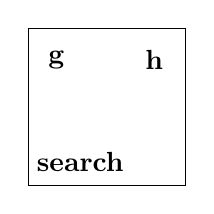
\begin{tikzpicture}[scale=1, transform shape]
\draw (0,0) rectangle (2,2);
\node at (0.66,0.3) {\textbf{search}};
\node at (0.36,1.6) {\textbf{g}};
\node at (1.6,1.6) {\textbf{h}};
\end{tikzpicture}
\caption{Legenda}
\label{fig:legenda}
\end{figure}


\begin{figure}[H]
\centering
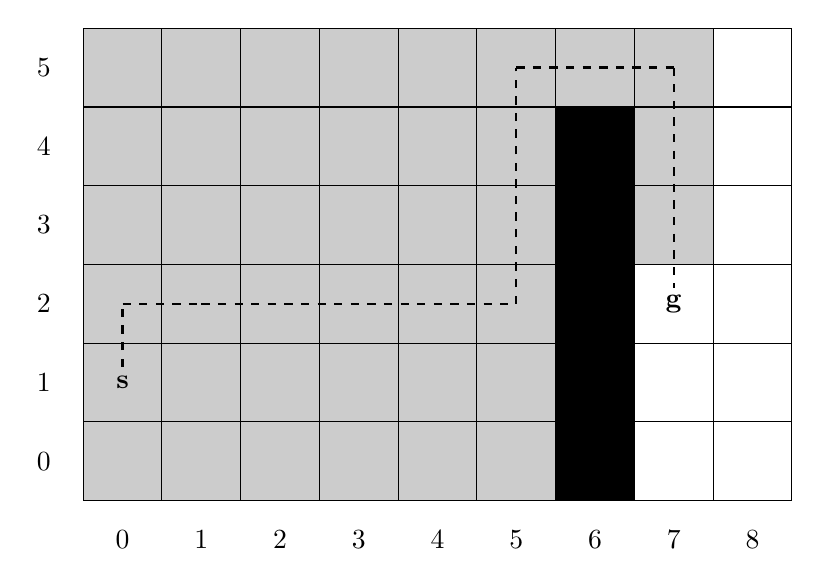
\begin{tikzpicture}[scale = 1, transform shape]
\fill [black!20!white] (0,0) rectangle  (6,6);
\fill [black!20!white] (7,3) rectangle  (6,6);
\fill [black!20!white] (7,3) rectangle  (8,6);
    \draw[step=1cm,black,thin] (0,0) grid (9,6);
    \foreach \xtick in {0,...,8} {\pgfmathsetmacro\result{\xtick * 1} \node at (\xtick+0.5, -.5) {\pgfmathprintnumber{\result}}; }
    \foreach \ytick in {5,4,3,2,1,0} {\pgfmathsetmacro\result{\ytick * 1} \node at (-.5,\ytick+0.5) {\pgfmathprintnumber{\result}}; }
    %\foreach \x/\y in {.5/2.5, 1.5/.5, 2.5/4.5, 3.5/1.5, 4.5/3.5}{\draw [fill=black, thin] (\x,\y);}
\fill[black] (6,0) rectangle (7,5);
\node at (+0.5, +1.5) {\textbf{s}};
\node at (7.5, 2.5) {\textbf{g}};

\populateCell{0}{1}{0}{8}{1}
\populateCell{0}{0}{1}{9}{1}
\populateCell{1}{0}{2}{8}{1}
\populateCell{2}{0}{3}{7}{1}
\populateCell{3}{0}{4}{6}{1}
\populateCell{4}{0}{5}{6}{1}
\populateCell{5}{0}{6}{4}{1}
\populateCell{1}{1}{1}{7}{1}
\populateCell{2}{1}{2}{6}{1}
\populateCell{3}{1}{3}{5}{1}
\populateCell{4}{1}{4}{4}{1}
\populateCell{5}{1}{5}{3}{1}
\populateCell{0}{2}{1}{7}{1}
\populateCell{1}{2}{2}{6}{1}
\populateCell{2}{2}{3}{5}{1}
\populateCell{3}{2}{4}{4}{1}
\populateCell{4}{2}{5}{3}{1}
\populateCell{5}{2}{6}{2}{1}
\populateCell{0}{3}{2}{8}{1}
\populateCell{1}{3}{3}{7}{1}
\populateCell{2}{3}{4}{6}{1}
\populateCell{3}{3}{5}{5}{1}
\populateCell{4}{3}{6}{4}{1}
\populateCell{5}{3}{7}{3}{1}
\populateCell{0}{4}{3}{9}{1}
\populateCell{1}{4}{4}{8}{1}
\populateCell{2}{4}{5}{7}{1}
\populateCell{3}{4}{6}{6}{1}
\populateCell{4}{4}{7}{5}{1}
\populateCell{5}{4}{8}{4}{1}
\populateCell{0}{5}{4}{10}{1}
\populateCell{1}{5}{5}{9}{1}
\populateCell{2}{5}{6}{8}{1}
\populateCell{3}{5}{7}{7}{1}
\populateCell{4}{5}{8}{6}{1}
\populateCell{5}{5}{9}{5}{1}
\populateCell{6}{5}{10}{4}{1}
\populateCell{7}{5}{11}{3}{1}
\populateCell{8}{5}{12}{4}{1}
\populateCell{8}{4}{13}{3}{1}
\populateCell{7}{4}{12}{2}{1}
\populateCell{7}{3}{13}{1}{1}
\populateCell{8}{3}{14}{2}{1}
\populateCell{7}{2}{14}{0}{1}
\populateCell{8}{2}{}{}{0}
\populateCell{8}{1}{}{}{0}
\populateCell{8}{0}{}{}{0}
\populateCell{7}{0}{}{}{0}
\populateCell{7}{1}{}{}{0}

\draw[black,thick,dashed] (0.5, 1.7) -- (0.5, 2.5);
\draw[black,thick,dashed] (0.5, 2.5) -- (1.5, 2.5);
\draw[black,thick,dashed] (1.5, 2.5) -- (5.5, 2.5);
\draw[black,thick,dashed] (5.5, 2.5) -- (5.5, 5.5);
\draw[black,thick,dashed] (5.5, 5.5) -- (7.5, 5.5);
\draw[black,thick,dashed] (7.5, 5.5) -- (7.5, 2.7);



\end{tikzpicture}   
\caption[caption]{LMTAA*: termine iterazione 1\\\hspace{\textwidth}$counter = 1$\\\hspace{\textwidth}$pathcost(1) = 14$\\\hspace{\textwidth}$deltah(1) = 0$} \label{fig:AA1}
\end{figure}
\par{Ia nodi $s_{start}$ (0,1) e $s_{goal}$ (7,2) vengono inizializzati prima di effettuare la ricerca (linee \ref{alg:aa2}-\ref{alg:aa3}). Visto che il loro valore search() \`e iniziamente pari a 0, si entrer\`a nel primo ramo condizionale della procedura InitializeState() (linea \ref{alg:aa18}). Al termine di tale procedura i nodi di partenza e di arrivo avranno valori h pari rispettivamente a 8 e 0, valori g pari a infinito e valore search pari a 1. Prima di chiamare la procedura principale ComputePath() viene corretto il valore g del nodo di partenza a 0. Partendo da una griglia in cui tutti gli valori g e h non sono stati inizializzati e tutti i valori search() sono nulli, comincia la ricerca nel modo usuale di A*.}
\par{Tutti i nodi successori vengono passati alla procedura InitializeState() dove verr\`a computato il loro valore h. Visto che si tratta della prima ricerca verr\`a eseguito il ramo condizionale sulla linea \ref{alg:aa18} e verr\`a inoltre memorizzato il loro valore search() a 1}
\par{A fine ricerca viene memorizzato il costo del percorso trovato nel mapping $pathcost(1)$ (linea \ref{alg:aa6}). A questo punto l'agent sorgente si muove lungo il percorso da (0,1) a (1,2).
L'agent  target si muove da (7,2) a (8,3), uscendo fuori dal percorso che l'agent sorgente aveva calcolato. L'esecuzione entrer\`a dunque nel ramo condizionale sulla linea \ref{alg:aa17}. Qui verr\`a inizializzato il nuovo nodo di arrivo per garantire che i suoi valori euristici siano \emph{coerenti} con con il nodo di arrivo precedente. Nel nostro caso, il nodo (8,3) \`e gi\`a stato scoperto in questa ricerca ed \`e gi\`a consitente verso il vecchio nodo di arrivo. L'esecuzione non entrer\`a pertanto in nessun ramo condizionale, uscendo dalla procedura InitializeState() senza aver apportato modifiche. L'esecuzione salta il ramo condizionale sulla linea \ref{alg:aa19} poich\`e non ci sono le condizioni, arrivando direttamente alla linea \ref{alg:aa12}. Qui, il valore di $deltah(x)$ durante la $x$-esima esecuzione, pu\`o considerarsi come la somma di tutte le correzioni effettuate fino all'inizio della $x$-esima ricerca. Si otterr\`a quindi deltah(2) = deltah(1) + h((8,3)) = 2. Infine verr\`a aggiornato il nodo di arrivo (linea \ref{alg:aa20}) e ricomincer\`a il loop principale.}
\par{
L'agent sorgente si vedr\`a dunque costretto a pianificare un nuovo percorso. Il termine della seconda iterazione \`e mostrata in figura \ref{fig:AA2}.} 
\begin{figure}[H]
\centering
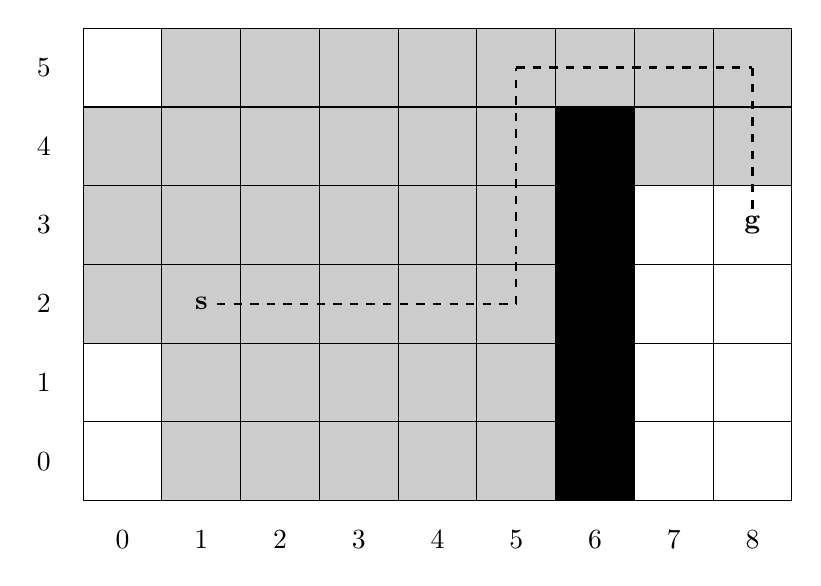
\begin{tikzpicture}

\fill [black!20!white] (1,0) rectangle  (6,6);
\fill [black!20!white] (0,2) rectangle  (1,5);
\fill [black!20!white] (4,5) rectangle  (9,6);
\fill [black!20!white] (7,4) rectangle  (9,5);

    \draw[step=1cm,black,thin] (0,0) grid (9,6);
    \foreach \xtick in {0,...,8} {\pgfmathsetmacro\result{\xtick * 1} \node at (\xtick+0.5, -.5) {\pgfmathprintnumber{\result}}; }
    \foreach \ytick in {5,4,3,2,1,0} {\pgfmathsetmacro\result{\ytick * 1} \node at (-.5,\ytick+0.5) {\pgfmathprintnumber{\result}}; }
    %\foreach \x/\y in {.5/2.5, 1.5/.5, 2.5/4.5, 3.5/1.5, 4.5/3.5}{\draw [fill=black, thin] (\x,\y);}
\fill[black] (6,0) rectangle (7,5);


\node at (+1.5, +2.5) {\textbf{s}};
\node at (8.5, 3.5) {\textbf{g}};

\populateCell{0}{1}{2}{12}{2}
\populateCell{0}{0}{3}{11}{2}
\populateCell{1}{0}{2}{10}{2}
\populateCell{2}{0}{3}{9}{2}
\populateCell{3}{0}{4}{8}{2}
\populateCell{4}{0}{5}{7}{2}
\populateCell{5}{0}{6}{6}{2}
\populateCell{1}{1}{2}{11}{2}
\populateCell{2}{1}{2}{10}{2}
\populateCell{3}{1}{3}{9}{2}
\populateCell{4}{1}{4}{8}{2}
\populateCell{5}{1}{5}{7}{2}
\populateCell{0}{2}{1}{11}{2}
\populateCell{1}{2}{0}{10}{2}
\populateCell{2}{2}{1}{9}{2}
\populateCell{3}{2}{2}{8}{2}
\populateCell{4}{2}{3}{7}{2}
\populateCell{5}{2}{4}{6}{2}
\populateCell{0}{3}{2}{10}{2}
\populateCell{1}{3}{1}{9}{2}
\populateCell{2}{3}{2}{8}{2}
\populateCell{3}{3}{3}{7}{2}
\populateCell{4}{3}{4}{6}{2}
\populateCell{5}{3}{5}{5}{2}
\populateCell{0}{4}{3}{9}{2}
\populateCell{1}{4}{2}{8}{2}
\populateCell{2}{4}{3}{7}{2}
\populateCell{3}{4}{4}{6}{2}
\populateCell{4}{4}{5}{5}{2}
\populateCell{5}{4}{6}{4}{2}
\populateCell{0}{5}{4}{10}{2}
\populateCell{1}{5}{3}{7}{2}
\populateCell{2}{5}{4}{8}{2}
\populateCell{3}{5}{5}{7}{2}
\populateCell{4}{5}{6}{6}{2}
\populateCell{5}{5}{7}{5}{2}
\populateCell{6}{5}{8}{4}{2}
\populateCell{7}{5}{9}{3}{2}
\populateCell{8}{5}{10}{2}{2}
\populateCell{8}{4}{11}{1}{2}
\populateCell{7}{4}{10}{2}{2}
\populateCell{7}{3}{11}{1}{2}
\populateCell{8}{3}{12}{0}{2}
\populateCell{7}{2}{14}{0}{1}
\populateCell{8}{2}{}{}{1}
\populateCell{8}{1}{}{}{1}
\populateCell{8}{0}{}{}{1}
\populateCell{7}{0}{}{}{1}
\populateCell{7}{1}{}{}{1}



\draw[black,thick,dashed] (1.7, 2.5) -- (5.5, 2.5);
\draw[black,thick,dashed] (5.5, 2.5) -- (5.5, 5.5);
\draw[black,thick,dashed] (5.5, 5.5) -- (8.5, 5.5);
\draw[black,thick,dashed] (8.5, 5.5) -- (8.5, 3.7);




\end{tikzpicture}   
\caption[caption]{LMTAA*: termine iterazione 2\\\hspace{\textwidth}$counter = 2$\\\hspace{\textwidth}$pathcost(2) = 12$\\\hspace{\textwidth}$deltah(2) = 2$} \label{fig:AA2}
\end{figure}
\par{All'inizio di questa esecuzione, gran parte dei nodi s hanno valore search(s) pari a 1 poich\'e sono stati esplorati nella ricerca precedente. Nel corpo della funzione ComputePath(), ogni qual volta viene chiamata la procedura InitializeState() su un successore s con valore search(s) = 1, l'esecuzione entrer\`a nel ramo condizionale sulla linea \ref{alg:aa22}.}
\par{In generale, se un nodo s \`e stato esplorato in una esecuzione precedente ($search(s) \neq 0$) ma non ancora esplorato nella ricerca corrente ($search(s) \neq counter$), allora Adaptive-A* aggiorna il suo valore h con la somma di tutte le correzioni tra l'esecuzione che in cui \`e stato inizializzato il nodo s l'ultima volta e l'esecuzione corrente. Questo valore \`e uguale a $deltah(counter) - deltah(search(s))$ (linea \ref{alg:aa8}). In questa iterazione in particolare, ci interesser\`a il fattore di correzione tra l'esecuzione corrente e l'esecuzione 1: $deltah(2) - deltah(1) = 2$. Viene poi scelto il massimo tra il valore euristico corretto con tale fattore di correzione e l'euristica fornita dall'utente per garantire la consistenza del nuovo valore h verso il nuovo nodo di arrivo (linea \ref{alg:aa9}).}
\par{Per alcuni nodi vale anche la condizione in linea \ref{alg:aa21}, che una volta inizializzati avranno un valore h particolarmente pi\`u accurato del precedente. Si veda ad esempio il nodo di coordinate (5,2), che aveva valore euristico pari a 2 nella prima esecuzione e alla fine della seconda sar\`a invece pari a 6.}
\par{Neanche qui sono visibili grandi vantaggi, a parte il fatto che le euristiche cominciano ad essere maggiormente accurate. Ci\`o vuol dire che ogni nodo sa con maggior precisione quanto dista dal nodo di goal. Pi\`u tale stima \`e accurata, meno saranno i nodi esplorati dalle ricerche future. A questo punto l'agent sorgente si muove da (1,2) a (2,2).  L'agent goal si muove da (8,3) a (7,3). Viene calcolato il valore $deltah(3)$ che sar\`a pari a $deltah(2) + h((7,3)) = 2 + 1 = 3$. L'agent sorgente dovr\`a pianificare un nuovo percorso per la terza volta. In figura \ref{fig:AA3} \`e mostrata la terza iterazione di LMTAA*.}
\begin{figure}[H]
\centering
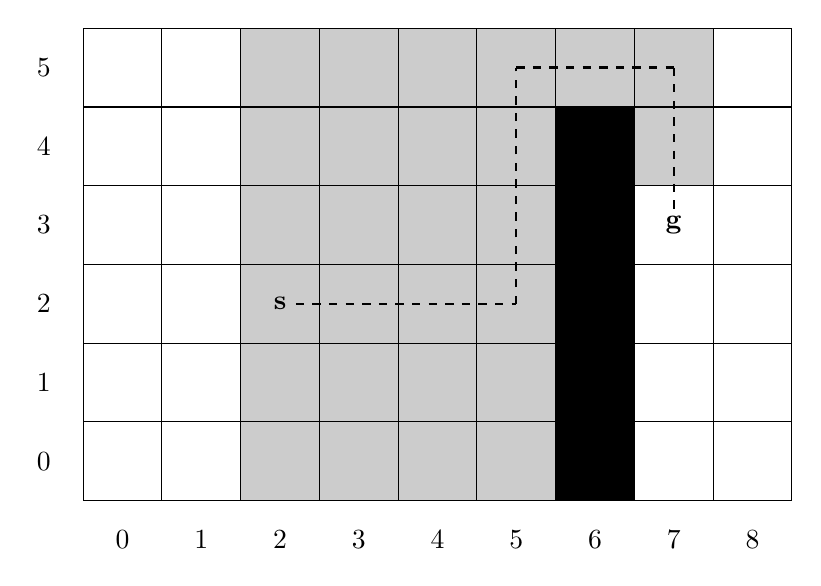
\begin{tikzpicture}

\fill [black!20!white] (2,0) rectangle  (6,6);
\fill [black!20!white] (6,4) rectangle  (8,6);


    \draw[step=1cm,black,thin] (0,0) grid (9,6);
    \foreach \xtick in {0,...,8} {\pgfmathsetmacro\result{\xtick * 1} \node at (\xtick+0.5, -.5) {\pgfmathprintnumber{\result}}; }
    \foreach \ytick in {5,4,3,2,1,0} {\pgfmathsetmacro\result{\ytick * 1} \node at (-.5,\ytick+0.5) {\pgfmathprintnumber{\result}}; }
    %\foreach \x/\y in {.5/2.5, 1.5/.5, 2.5/4.5, 3.5/1.5, 4.5/3.5}{\draw [fill=black, thin] (\x,\y);}
\fill[black] (6,0) rectangle (7,5);


\node at (+2.5, +2.5) {\textbf{s}};
\node at (7.5, 3.5) {\textbf{g}};

\populateCell{0}{1}{2}{12}{2}
\populateCell{0}{0}{3}{11}{2}
\populateCell{1}{0}{3}{9}{3}
\populateCell{2}{0}{2}{8}{3}
\populateCell{3}{0}{3}{7}{3}
\populateCell{4}{0}{4}{6}{3}
\populateCell{5}{0}{5}{5}{3}
\populateCell{1}{1}{2}{11}{3}
\populateCell{2}{1}{1}{9}{3}
\populateCell{3}{1}{2}{8}{3}
\populateCell{4}{1}{3}{7}{3}
\populateCell{5}{1}{4}{6}{3}
\populateCell{0}{2}{1}{11}{2}
\populateCell{1}{2}{1}{11}{3}
\populateCell{2}{2}{0}{10}{3}
\populateCell{3}{2}{1}{9}{3}
\populateCell{4}{2}{2}{8}{3}
\populateCell{5}{2}{3}{7}{3}
\populateCell{0}{3}{2}{10}{2}
\populateCell{1}{3}{2}{10}{3}
\populateCell{2}{3}{1}{9}{3}
\populateCell{3}{3}{2}{8}{3}
\populateCell{4}{3}{3}{7}{3}
\populateCell{5}{3}{4}{6}{3}
\populateCell{0}{4}{3}{9}{2}
\populateCell{1}{4}{3}{9}{3}
\populateCell{2}{4}{2}{8}{3}
\populateCell{3}{4}{3}{7}{3}
\populateCell{4}{4}{4}{6}{3}
\populateCell{5}{4}{5}{5}{3}
\populateCell{0}{5}{4}{10}{2}
\populateCell{1}{5}{4}{8}{3}
\populateCell{2}{5}{3}{7}{3}
\populateCell{3}{5}{4}{6}{3}
\populateCell{4}{5}{5}{5}{3}
\populateCell{5}{5}{6}{4}{3}
\populateCell{6}{5}{7}{3}{3}
\populateCell{7}{5}{8}{2}{3}
\populateCell{8}{5}{9}{3}{3}
\populateCell{8}{4}{10}{2}{3}
\populateCell{7}{4}{9}{1}{3}
\populateCell{7}{3}{10}{0}{3}
\populateCell{8}{3}{12}{0}{2}
\populateCell{7}{2}{14}{0}{1}
\populateCell{8}{2}{}{}{1}
\populateCell{8}{1}{}{}{1}
\populateCell{8}{0}{}{}{1}
\populateCell{7}{0}{}{}{1}
\populateCell{7}{1}{}{}{1}



\draw[black,thick,dashed] (2.7, 2.5) -- (5.5, 2.5);
\draw[black,thick,dashed] (5.5, 2.5) -- (5.5, 5.5);
\draw[black,thick,dashed] (5.5, 5.5) -- (7.5, 5.5);
\draw[black,thick,dashed] (7.5, 5.5) -- (7.5, 3.7);




\end{tikzpicture}   
\caption[caption]{LMTAA*: termine iterazione 3\\\hspace{\textwidth}$counter = 3$\\\hspace{\textwidth}$pathcost(3) = 10$\\\hspace{\textwidth}$deltah(3) = 3$} \label{fig:AA3}
\end{figure}
\par{ A questo punto le euristiche sono abbastanza informate. Gran parte dei nodi sanno esattamente quanto distano realmente dal nodo di arrivo. Solo in questa ultima iterazione, sono stati esplorati 27 nodi. Per rendere ben chiari i vantaggi di LMTAA* \`e stata mostrata, in figura \ref{fig:A3}, la stessa identica situazione di questa ultima iterazione con la differenza sostanziale che l'agent $s$ si avvale di A* tradizionale e quindi di euristiche \textbf{non} informate.}

\begin{figure}[H]
\centering
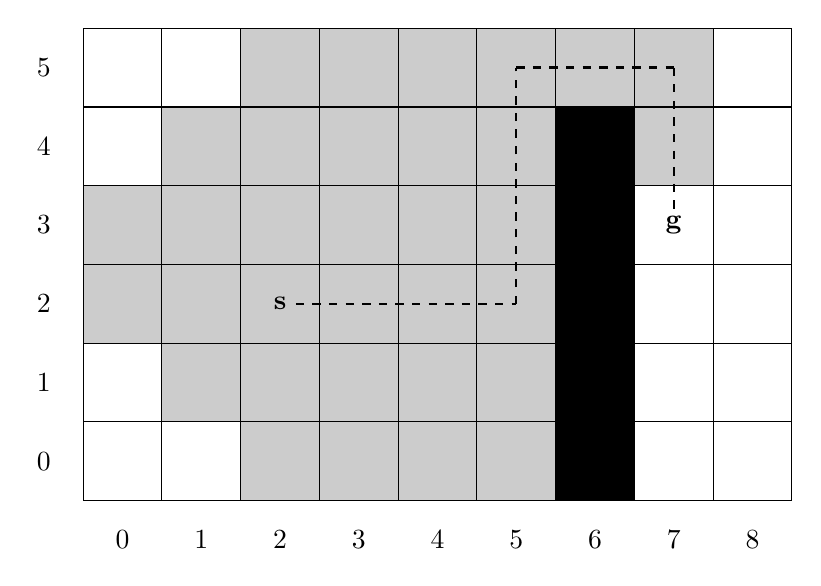
\begin{tikzpicture}

\fill [black!20!white] (0,2) rectangle  (6,4);
\fill [black!20!white] (1,1) rectangle  (6,5);
\fill [black!20!white] (2,0) rectangle  (6,6);
\fill [black!20!white] (6,4) rectangle  (8,6);


    \draw[step=1cm,black,thin] (0,0) grid (9,6);
    \foreach \xtick in {0,...,8} {\pgfmathsetmacro\result{\xtick * 1} \node at (\xtick+0.5, -.5) {\pgfmathprintnumber{\result}}; }
    \foreach \ytick in {5,4,3,2,1,0} {\pgfmathsetmacro\result{\ytick * 1} \node at (-.5,\ytick+0.5) {\pgfmathprintnumber{\result}}; }
    %\foreach \x/\y in {.5/2.5, 1.5/.5, 2.5/4.5, 3.5/1.5, 4.5/3.5}{\draw [fill=black, thin] (\x,\y);}
\fill[black] (6,0) rectangle (7,5);


\node at (+2.5, +2.5) {\textbf{s}};
\node at (7.5, 3.5) {\textbf{g}};

\populateCell{0}{1}{3}{9}{3}
\populateCell{0}{0}{}{}{2}
\populateCell{1}{0}{3}{9}{3}
\populateCell{2}{0}{2}{8}{3}
\populateCell{3}{0}{3}{7}{3}
\populateCell{4}{0}{4}{6}{3}
\populateCell{5}{0}{5}{5}{3}
\populateCell{1}{1}{2}{8}{3}
\populateCell{2}{1}{1}{7}{3}
\populateCell{3}{1}{2}{6}{3}
\populateCell{4}{1}{3}{5}{3}
\populateCell{5}{1}{4}{4}{3}
\populateCell{0}{2}{2}{8}{3}
\populateCell{1}{2}{1}{7}{3}
\populateCell{2}{2}{0}{6}{3}
\populateCell{3}{2}{1}{5}{3}
\populateCell{4}{2}{2}{4}{3}
\populateCell{5}{2}{3}{3}{3}
\populateCell{0}{3}{3}{7}{3}
\populateCell{1}{3}{2}{6}{3}
\populateCell{2}{3}{1}{5}{3}
\populateCell{3}{3}{2}{4}{3}
\populateCell{4}{3}{3}{3}{3}
\populateCell{5}{3}{4}{2}{3}
\populateCell{0}{4}{4}{8}{3}
\populateCell{1}{4}{3}{7}{3}
\populateCell{2}{4}{2}{6}{3}
\populateCell{3}{4}{3}{5}{3}
\populateCell{4}{4}{4}{4}{3}
\populateCell{5}{4}{5}{3}{3}
\populateCell{0}{5}{}{}{2}
\populateCell{1}{5}{4}{8}{3}
\populateCell{2}{5}{3}{7}{3}
\populateCell{3}{5}{4}{6}{3}
\populateCell{4}{5}{5}{5}{3}
\populateCell{5}{5}{6}{4}{3}
\populateCell{6}{5}{7}{3}{3}
\populateCell{7}{5}{8}{2}{3}
\populateCell{8}{5}{9}{3}{3}
\populateCell{8}{4}{10}{2}{3}
\populateCell{7}{4}{9}{1}{3}
\populateCell{7}{3}{10}{0}{3}
\populateCell{8}{3}{}{}{2}
\populateCell{7}{2}{}{}{1}
\populateCell{8}{2}{}{}{1}
\populateCell{8}{1}{}{}{1}
\populateCell{8}{0}{}{}{1}
\populateCell{7}{0}{}{}{1}
\populateCell{7}{1}{}{}{1}



\draw[black,thick,dashed] (2.7, 2.5) -- (5.5, 2.5);
\draw[black,thick,dashed] (5.5, 2.5) -- (5.5, 5.5);
\draw[black,thick,dashed] (5.5, 5.5) -- (7.5, 5.5);
\draw[black,thick,dashed] (7.5, 5.5) -- (7.5, 3.7);




\end{tikzpicture}   
\caption[caption]{Plain A*: termine iterazione 3} \label{fig:A3}
\end{figure}

\par {A* esplorerebbe 33 nodi, contro i 27 di LMTAA*. A causa delle modeste dimensioni di tale esempio non si pu\`o apprezzare una grande differenza, ma si pensi a situazioni in cui un agent deve ripianificare continuamente un percorso verso un altro agent in una griglia con dimensioni superiori di diversi ordini di potenza e in cui il runtime di una singola ricerca \`e un fattore critico per il funzionamento del sistema. In questo caso un algoritmo di ricerca incrementale \`e senza dubbio preferibile per via del suo vantaggio di migliorare le proprie prestazioni al crescere delle iterazioni.}
\section{Trailmax}
\label{sec:trailmax}

\par{Il problema del \emph{moving target search} (noto anche come \emph{pursuit-evasion} o in italiano \emph{guardie e ladri}) \`e una famiglia di problemi gi\`a noti alla matematica e all'informatica, ed ha molte applicazioni in particolar modo ai videogiochi.
}
\par{Spesso nei videogiochi il giocatore controlla un ladro che deve sfuggire ad un poliziotto a sua volta controllato da una intelligenza artificiale. Tuttavia non \`e raro che lo stesso gioco venga capovolto, ad esempio in modo che il giocatore controlli il poliziotto e che il ladro controllato da una intelligenza artificiale cerchi di sfuggirgli.}
\par{Visto che tutti gli algoritmi descritti fin'ora sono applicabili solo all'inseguimento, si \`e reso necessario lo sviluppo di un algoritmo utile per definire una strategia di evasione per il target. In questo capitolo verr\`a dunque introdotto un algoritmo che risponde a questa esigenza, chiamato TrailMax\footnote{Evaluating Strategies for Running from the Cops, Carsten Moldenhauer
and
Nathan R. Sturtevant
Department of Computer Science
University of Alberta
Edmonton, AB, Canada T6G 2E8}.
}\par{Per semplicit\`a nella descrizione dell'algoritmo assumeremo che i due agent abbiano la stessa velocit\`a. Tuttavia tutte le seguenti definizioni sono estendibili anche a differenti velcit\`a. L'idea di fondo di questo algoritmo \`e che il target assume che l'inseguitore sappia in anticipo qual \`e il percorso migliore per raggiungerlo. Partendo da questa assunzione il target prova a massimizzare il tempo di cattura, scegliendo quindi un percorso che impiegher\`a all'inseguitore pi\`u tempo per raggiungere l'obiettivo.}
\par{Il percorso di evasione \`e calcolato espandendo simultaneamente i nodi intorno alla posizione dell'inseguitore e del target utilizzando una variante dell'algoritmo di Dijkstra. Vi saranno pertanto due code di priorit\`a, una per l'inseguitore e una per il target. Ogni nodo esplorato dal target \`e confrontato con quelli esplorati dall'inseguitore al fine di controllare se l'inseguitore potrebbe gi\`a aver raggiunto quel nodo e catturato il target. Se \`e questo il caso, il nodo viene scartato. In caso contrario tale nodo appartiene alla copertura del target e pertanto espanso normalmente. Invece, i nodi presenti nella coda di priorit\`a dell'inseguitore sono sempre esplorati normalmente. Nella figura \ref{trailmaxexp} \`e mostrata una rappresentazione dell'espansione di TrailMax. L'area grigia contiene nodi che sono stati raggiunti per prima dal target, dichiarati come copertura del target, ma che non sono pi\`u stati espansi siccome sono stati catturati in seguito dall'inseguitore}
\begin{figure}[htp]
\centering
\includegraphics[scale=0.80]{/home/notsaved/2017-08-03-214425_438x196_scrot.png}
\caption{Visualizzazione della computazione di TrailMax.}
\label{trailmaxexp}
\end{figure}
\par{L'algoritmo termina quando tutti i nodi appartenenti alla copertura del target sono espansi anche dall'inseguitore. L'ultimo nodo esplorato dall'inseguitore sar\`a il nodo che il target dovr\`a raggiungere. Il percorso viene generato percorrendo a ritroso tutte le connessioni usate per arrivare a tale nodo, fino a raggiungere il nodo di partenza.}
\iffalse\begin{figure}[htp]
\centering
\includegraphics[scale=0.40]{/home/notsaved/theta2.png}
\caption{Il percorso mostrato in verde \`e quello calcolato da Trailmax}
\label{trail1}
\end{figure}
\fi


\begin{figure}[H]
\minipage{0.42\textwidth}
  \includegraphics[width=\linewidth]{/home/notsaved/theta2.png}
  \caption{TrailMax su mappa outdoor}
  \label{fig:trailmax_outdoor}
\endminipage\hfill
\minipage{0.42\textwidth}%
  \includegraphics[width=\linewidth]{/home/notsaved/theta3.png}
  \caption{TrailMax su mappa indoor}\label{fig:trailmax_indoor}
\endminipage
\caption{Le immagini mostrano il percorso calcolato da TrailMax (verde) che massimizza la distanza dall'agent inseguitore (Rosso)}
\end{figure}

\chapter{Design ed Implementazione}
\par{L'implementazione del framework \`e stata realizzata in linguaggio Java. La definizione delle classi dei grafi \`e fornita dalla libreria JGrapht\footnote{jgrapht.org: JGraphT is a free Java graph library that provides mathematical graph-theory objects and algorithms}. }
\par{In questo capitolo saranno inoltre descritte le classi che compongono il framework con relativi dettagli implementativi e le loro interazioni.}
\section{Logica di gioco e gestione input}
\par{La classe Game ha la responsabilit\`a di gestire le informazioni sullo stato di gioco. \`E la classe del gioco che implementa il game loop nel metodo \emph{gameLoop()}. In tale metodo si svolge la logica del gioco. Il game loop \`e sempre in esecuzione durante il gameplay e ad ogni iterazione processa l'input dell'utente, aggiorna lo stato di gioco e infine \emph{renderizza} gli elementi di gioco. Tiene inoltre traccia del lasso di tempo che impiega una singola iterazione del ciclo per controllare il \emph{framerate}.}
\par{Durante l'inizializzazione del gioco vengono instanziate le classi Player e GameController. La classe player mantiene le informazioni sullo stato del giocatore ed espone dei metodi utili a ricavarne la posizione sul terreno di gioco e per muoverlo all'interno di quest'ultima. La classe GameController implementa l'interfaccia java \emph{KeyListener} e gestisce gli input da tastiera e controlla gli spostamenti del giocatore similmente al \emph{design pattern} MVC. Questa classe ha la responsabilit\`a di aggiornare la posizione del giocatore in base a un lasso di tempo \emph{delta} calcolato nel game loop e ai tasti premuti dall'utente.}

\begin{figure}[htp]
\centering
\includegraphics[scale=0.50]{/home/notsaved/Documenti/game_controller.png}
\caption{Classi Game, GameController e Player}
\label{gamecontroller}
\end{figure}

\section{Ambiente di gioco}
\begin{figure}[H]
\centering
\includegraphics[scale=0.50]{/home/notsaved/Documenti/GameMap_MapGen.png}
\caption{Classi GameMap, MapGenerator e TileMapElement}
\label{gamemapclass}
\end{figure}
\par{La classe GameMap \`e responsabile della definizione dell'ambiente di gioco. Come accennato nei capitoli precedenti, l'ambiente di gioco si basa su una griglia di dimensioni fissate (WIDTH e HEIGHT) di oggetti Tile. La classe Tile definisce un singolo tassello che andr\`a a comporre la mappa ed espone un unico metodo che ritorna il proprio stato booleano. Definisce inoltre la dimensione standard di ogni singolo tassello nella costante statica TILE\_SIZE.}
\par{Il costruttore della classe GameMap riceve in ingresso un oggetto di tipo MapGenerator. Come si vede nella figura \ref{gamemapclass}, MapGenerator \`e una interfaccia, le cui sottoclassi implementano il vero algoritmo di costruzione della mappa, secondo il design pattern \emph{Strategy}. Sar\`a pertanto responsabilit\`a di una delle sottoclassi di MapGenerator di definire la morfologia dell'ambiente di gioco cambiando lo stato dei tile della griglia. In tal modo si possono facilmente implementare nuove tipologie di mappe semplicemente estendendo tale interfaccia e facendo overriding sul metodo \emph{generate()}. I generatori di mappe Outdoor e Dungeon in particolare instanziano degli oggetti che estendono la classe astratta TileMapElement, rispettivamente Obstacle e Room, delle quali viene mantenuto un riferimento nella classe GameMap per facilitare la costruzione della morfologia di tali tipi di mappa come vedremo nel capitolo successivo.}
\par{Una volta costruita la morfologia della mappa, viene costruito il suo grafo di navigazione partendo da un grafo inizialmente vuoto. Vengono poi instanziati ed aggiunti al grafo degli oggetti di tipo Node per ogni cella non bloccata. Gli oggetti di tipo Node sono identificati da un intero secondo lo schema visto nella sezione \ref{subs:griglie} per convertire facilmente il numero che identifica il nodo nelle sue coordinate geometriche sulla griglia. Infine, per ogni nodo instanziato si controllano le coordinate geometriche delle celle adiacenti e se il loro stato non \`e bloccato allora viene instanziato e aggiunto al grafo un oggetto di tipo Edge che rappresenta un arco tra due nodi e con peso unitario se si tratta di un arco ortogonale o $\sqrt2$ se si tratta di un arco diagonale.}
\par{La classe GameMap espone inoltre alcuni metodi utili a verificare ad esempio se una certa coordinata \`e bloccata o meno, metodi \emph{getter} per ottenere la griglia o il grafo, metodi per aggiungere ostacolo o stanze (usati solo dai relativi generatori) ed in fine un metodo statico che controlla se due punti sulla mappa sono in linea di visibilit\`a o meno.}

\section{Entit\`a e comportamento}
\begin{figure}[htp]
\centering
\includegraphics[scale=0.50]{/home/notsaved/Documenti/Entity_Behaviour.png}
\caption{Classe Entity e Behaviour}
\label{entity_behaviour}
\end{figure}
\par{La classe Entity definisce ogni agent all'interno dell'intero sistema di gioco, rendendola una delle classi pi\`u importanti dell'intero sistema. Tra i suoi attributi vi sono alcune costanti che definisconono la velocit\`a e il raggio di collisione, la posizione espressa in coordinate geometriche, l'immagine da renderizzare sulla mappa, un riferimento alla mappa di gioco e un oggetto di tipo Behaviour. La classe Entity rappresenta solamente il modello di una entit\`a. Infatti le funzionalit\`a di cervello pensante, e quindi di controller, di ciascuna entit\`a sono delegate ad un oggetto che estende la classe astratta Behaviour. Applicando il design pattern Strategy sulla classe astratta Behaviour \`e possibile definire molteplici comportamenti per un Entity. Similmente alla classe Player, attraverso il metodo \emph{update}() che riceve in ingresso la grandezza di un lasso di tempo delta calcolato nel game loop verr\`a calcolato lo spostamento di un Entity.}
\par{Il comportamento di un Entity sar\`a dunque definito in una sottoclasse di Behaviour facendo \emph{overriding} sul metodo \emph{doBehaviour}(). Tale metodo viene chiamato ogni volta che dal game loop si richiede che l'entit\`a venga aggiornata. La classe mantiene inoltre un riferimento ad un oggetto \emph{Pathfinder}, che potr\`a variare a seconda del tipo effettivo della classe Behaviour.}
\par{Sono stati implementati due tipi di comportamento che una unit\`a di gioco pu\`o assumere rispetto al giocatore (o se si vuole rispetto a un'altra Entity) rispettivamente ChaseBehaviour ed EvadeBehaviour. La classe ChaseBehaviour definisce un comportamento di inseguimento di un Entity rispetto il giocatore. Utilizza di default come pathfinder una istanza di \emph{LazyMovingAdaptiveAStar}. Mantiene inoltre una flag booleana che indica se l'Entity ha raggiunto l'obiettivo ed in tal caso smette di muovere l'Entity. La classe EvadeBehaviour definisce invece un comportamento di evasione di un Entity rispetto il giocatore. Utilizza di default come pathfinder una istanza di \emph{Trailmax}. Mantiene inoltre una flag di stato che indica se l'Entity \`e stato raggiunto dal giocatore e in tal caso smette di muovere l'unit\`a di gioco.}

\section{Pathfinder}
\par{Le classi in figura \ref{classpathfinder} rappresentano e definiscono gli algoritmi descritti nel capitolo precedente. Tutti gli algoritmi di ricerca sviluppati nel framework implementano l'interfaccia pathfinder e fanno overriding sul metodo \emph{getShortestPath}(), nel quale risiede l'implementazione vera e propria dell'algoritmo in questione e che ritorna una lista di nodi che compongono il percorso trovato. Per gestire la priorit\`a dei nodi da processare (la coda Open) \`e stata utilizzata una implementazione della struttura dati \emph{FibonacciHeap}, fornita dalla libreria JGrapht. Per tener traccia dei nodi predecessori (cameFrom) e dei valori g() sono state utilizzate delle HashMap. Infine sono stati usati degli HashSet per i nodi processati (Closed).}
\begin{figure}[htp]
\centering
\includegraphics[scale=0.45]{/home/notsaved/Documenti/PathfinderClass.png}
\caption{Classi Pathfinder}
\label{classpathfinder}
\end{figure}

\iffalse\begin{figure}[htp]
\centering
\includegraphics[width=\textwidth,height=\textheight,keepaspectratio,angle=270,origin=c]{/home/notsaved/ClassDiagramProgetto.jpg}
\caption{Class Diagram}
\label{classdiagram}
\end{figure}


\section{Game}
\begin{figure}[H]
\centering
\includegraphics[scale=0.80]{/home/notsaved/ClassDiagramProgettoGAME.jpg}
\caption{Classe Game}
\label{clssgame}
\end{figure}
La classe \emph{Game} mantiene le informazioni sullo stato del gioco, i riferimenti del giocatore e del relativo \emph{controller}, delle entit\`a instanziate e della mappa corrente. Inoltre implementa il \emph{loop} principale all'interno del quale avviene la logica del gioco e il \emph{rendering} degli elementi in gioco.

\section{Player}
\begin{figure}[H]
\centering
\includegraphics[scale=0.80]{/home/notsaved/ClassDiagramProgettoPLAYER.jpg}
\caption{Classe Player}
\label{clssplyr}
\end{figure}

La classe \emph{Player} mantiene le informazioni sullo stato del giocatore, la sua posizione sul terreno di gioco, velocit\`a di spostamento e immagine da renderizzare.

\section{Game Controller}
\begin{figure}[H]
\centering
\includegraphics[scale=0.80]{/home/notsaved/ClassDiagramProgettoCONTROLLER.jpg}
\caption{Classe GameController}
\label{gameController}
\end{figure}

La classe \emph{GameController} implementa l'interfaccia \emph{KeyListener} e gestisce gli input da tastiera, aggiornando in tal modo la posizione del giocatore, del quale mantiene un riferimento, similmente al \emph{design pattern} MVC.

\section{Tile}
\begin{figure}[H]
\centering
\includegraphics[scale=0.80]{/home/notsaved/ClassDiagramProgettoTILE.jpg}
\caption{Classe Tile}
\label{clssTile}
\end{figure}

La classe Tile rappresenta la pi\`u piccola unit\`a che compone una mappa di gioco. Questa classe mantiene una variabile di stato che indica se il tile \`e bloccato e una costante statica che indica la grandezza di ciascun tile.

\section{GameMap}
\begin{figure}[H]
\centering
\includegraphics[scale=0.80]{/home/notsaved/ClassDiagramProgettoGAMEMAP.jpg}
\caption{Classe GameMap}
\label{gamemap}
\end{figure}

La classe \emph{GameMap} si occupa di definire la geometria della mappa di gioco, mantenendo un riferimento di un array bidimensionale di oggetti Tile. Mantiene inoltre i riferimenti di eventuali stanze o ostacoli presenti sulla mappa. La geometria della mappa viene definita attraverso un oggetto che estende l'interfaccia \emph{MapGenerator}, di cui viene mantenuto il riferimento all'interno della classe GameMap, e facendo uso del design pattern \emph{Strategy} viene scelta la tipologia di mappa desiderata. Si occupa infine di generare il grafo associato a quella mappa basandosi sulla sua geometria.

\section{TileMapElement}
\begin{figure}[H]
\centering
\includegraphics[scale=0.80]{/home/notsaved/ClassDiagramProgettoTILEMAPELEMENT.jpg}
\caption{Classe TileMapElement}
\label{tilemapelement}
\end{figure}

Classe astratta che definisce un elemento generico sulla mappa di gioco. Gli attributi x e y ne determinano il posizionamento sull'area di gioco.

\section{Room}

\begin{figure}[H]
\centering
\includegraphics[scale=0.80]{/home/notsaved/ClassDiagramProgettoROOM.jpg}
\caption{Classe Room}
\label{classroom}
\end{figure}

La classe \emph{Room} estende la classe TileMapElement di cui sopra, ed \`e dotata di due attributi aggiuntivi che ne determinano l'altezza e la larghezza. In questo caso gli attributi x e y della superclasse TileMapElement si riconducono al Tile dell'angolo in basso a sinistra del rettangolo che la classe definisce. I Tile che appartengono al rettangolo definito dalla classe Room sono tutti traversabili. La classe \`e inoltre dotata di un metodo \emph{intersect}(), il quale restituisce true sse si verifica un \emph{overlapping} con un altro oggetto Room in ingresso.

\section{Obstacle}
\begin{figure}[H]
\centering
\includegraphics[scale=0.80]{/home/notsaved/ClassDiagramProgettoOBSTACLE.jpg}
\caption{Classe Obstacle}
\label{classobstacle}
\end{figure}

Similmente alla classe Room, la classe \emph{Obstacle} definisce un rettangolo di Tile ma in questo caso \emph{non} traversabili.

\section{MapGenerator}
\begin{figure}[H]
\centering
\includegraphics[scale=1.00]{/home/notsaved/ClassDiagramProgettoMAPGENERATOR.jpg}
\caption{Classe MapGenerator}
\label{classmapgenerator}
\end{figure}

Classe astratta che definisce un generico generatore di mappe.

\section{IndoorMapGenerator}

\begin{figure}[H]
\centering
\includegraphics[scale=0.80]{/home/notsaved/ClassDiagramProgettoINDOOR.jpg}
\caption{Classe IndoorMapGenerator}
\label{Classe IndoorMapGenerator}
\end{figure}

La classe \emph{IndoorMapGenerator} estende la classe astratta \emph{MapGenerator}. La costruzione della mappa \emph{indoor} avviene nel metodo \emph{generate()}, che fa a sua volta \emph{overriding} sul metodo astratto della superclasse. L'algoritmo per la generazione di mappe indoor sar\`a descritto dettagliatamente in una sezione successiva. 

\section{OutdoorMapGenerator}

\begin{figure}[H]
\centering
\includegraphics[scale=0.80]{/home/notsaved/ClassDiagramProgettoOUTDOOR.jpg}
\caption{Classe OutdoorMapGenerator}
\label{classoutdoorgenerator}
\end{figure}

La classe \emph{OutdoorMapGenerator} estende la classe astratta \emph{MapGenerator}. La costruzione della mappa \emph{outdoor} avviene nel metodo \emph{generate()}, che fa a sua volta \emph{overriding} sul metodo astratto della superclasse. L'algoritmo per la generazione di mappe outdoor sar\`a descritto dettagliatamente in una sezione successiva. 

\section{DungeonMapGenerator}

\begin{figure}[H]
\centering
\includegraphics[scale=0.80]{/home/notsaved/ClassDiagramProgettoDUNGEON.jpg}
\caption{Classe DungeonMapGenerator}
\label{classdungeonmap}
\end{figure}

La classe \emph{DungeonMapGenerator} estende la classe astratta \emph{MapGenerator}. La costruzione della mappa \emph{dungeon} avviene nel metodo \emph{generate()}, che fa a sua volta \emph{overriding} sul metodo astratto della superclasse. L'algoritmo per la generazione di mappe dungeon sar\`a descritto dettagliatamente in una sezione successiva. 

\section{Entity}

\begin{figure}[H]
\centering
\includegraphics[scale=0.80]{/home/notsaved/ClassDiagramProgettoENTITY.jpg}
\caption{Classe Entity}
\label{classentity}
\end{figure}

La classe \emph{Entity} definisce ogni agent all'interno dell'intero sistema di gioco, rendendola una delle classi pi\`u importanti dell'intero sistema. Essa tuttavia rappresenta solamente il \emph{modello} di una entit\`a. Infatti le funzionalit\`a di cervello pensante, e quindi di \emph{controller}, di ciascuna entit\`a sono delegate ad un oggetto che estende la classe astratta \emph{Behaviour} di cui si mantiene il riferimento all'interno della classe in esame. Attraverso il design pattern \emph{Strategy} sulla classe astratta Behaviour \`e possibile definire molteplici comportamenti per un Entity che esamineremo pi\`u dettagliatamente in una sezione successiva. Attraverso il metodo \emph{update}(), che riceve in ingresso la grandezza di un lasso di tempo, viene calcolato lo spostamento di un Entity.

\section{Behaviour}

\begin{figure}[H]
\centering
\includegraphics[scale=0.80]{/home/notsaved/ClassDiagramProgettoBEHAVIOUR.jpg}
\caption{Classe Behaviour}
\label{classbehaviour}
\end{figure}

Classe astratta che definisce un comportamento generico per un Entity. Le sue sottoclassi rappresentano il cervello di un Entity e si occupano di deciderne gli spostamenti, fungendo quindi da controller. Il comportamento di un Entity sar\`a dunque definito in una sua sottoclasse facendo \emph{overriding} sul metodo \emph{doBehaviour}(). La classe mantiene inoltre un riferimento ad un oggetto \emph{Pathfinder}, che potr\`a variare a seconda del tipo effettivo della classe Behaviour.

\section{ChaseBehaviour}

\begin{figure}[H]
\centering
\includegraphics[scale=0.80]{/home/notsaved/ClassDiagramProgettoCHASEBEHAVIOUR.jpg}
\caption{Classe ChaseBehaviour}
\label{classchase}
\end{figure}

La classe \emph{ChaseBehaviour} estende la classe Behaviour e definisce un comportamento di inseguimento di un Entity rispetto un Player oppure un altro Entity. Utilizza di default come pathfinder una istanza di \emph{LazyMovingAdaptiveAStar}. Mantiene inoltre una \emph{flag} di stato che indica se l'Entity ha raggiunto l'obiettivo ed in tal caso smette di muovere l'Entity.

\section{FleeBehaviour}

\begin{figure}[htp]
\centering
\includegraphics[scale=0.80]{/home/notsaved/ClassDiagramProgettoEVADEBEHAVIOUR.jpg}
\caption{Classe EvadeBehaviour}
\label{classevade}
\end{figure}

La classe \emph{FleeBehaviour} estende la classe Behaviour e definisce un comportamento di evasione di un Entity rispetto un Player oppure un altro Entity. Utilizza di default come pathfinder una istanza di \emph{Trailmax}. Mantiene inoltre una flag di stato che indica se l'Entity \`e stato raggiunto dal giocatore o dall'Entity dal quale si sta scappando. In tal caso smette di muovere l'Entity.

\section{Pathfinder}

\begin{figure}[H]
\centering
\includegraphics[scale=0.80]{/home/notsaved/ClassDiagramProgettoPATHFINDER.jpg}
\caption{Classe Pathfinder}
\label{classpathfind}
\end{figure}

Classe astratta che definisce un pathfinder generico. Le sue sottoclassi che implementano un algoritmo di pathfinding dovranno fare overriding sul metodo astratto \emph{getShortestPath}() il quale ritorna una lista di nodi che compongono il percorso trovato.

\section{Dijkstra}

\begin{figure}[H]
\centering
\includegraphics[scale=0.80]{/home/notsaved/ClassDiagramProgettoDIJKSTRA.jpg}
\caption{Classe Dijkstra}
\label{classdijkstra}
\end{figure}

La classe \emph{Dijkstra} estende la classe astratta \emph{Pathfinder} ed implementa una versione dell'omonimo algoritmo di cui ne abbiamo gi\`a ampiamente discusso nella sezione \ref{sec:dijkstra}.

\section{AStar}

\begin{figure}[H]
\centering
\includegraphics[scale=0.80]{/home/notsaved/ClassDiagramProgettoASTAR.jpg}
\caption{Classe AStar}
\label{classastar}
\end{figure}

La classe \emph{AStar} estende la classe astratta Pathfinder ed implementa una versione dell'omonimo algoritmo di cui ne abbiamo gi\`a ampiamente discusso nella sezione \ref{sec:astar}

\section{ThetaStar}

\begin{figure}[H]
\centering
\includegraphics[scale=0.80]{/home/notsaved/ClassDiagramProgettoTHETA.jpg}
\caption{Classe ThetaStar}
\label{classtheta}
\end{figure}

La classe \emph{ThetaStar} estende la classe astratta Pathfinder ed implementa una versione dell'omonimo algoritmo di cui ne abbiamo gi\`a ampiamente discusso nella sezione \ref{sec:theta}

\section{BidirectionalAStar}

\begin{figure}[H]
\centering
\includegraphics[scale=0.80]{/home/notsaved/ClassDiagramProgettoBIDIRECTIONAL.jpg}
\caption{Classe BidirectionalAStar}
\label{classbidirectional}
\end{figure}

La classe \emph{BidirectionalAStar} estende la classe astratta Pathfinder ed implementa una versione dell'omonimo algoritmo di cui ne abbiamo gi\`a ampiamente discusso nella sezione \ref{sec:bidirectional}

\section{LazyMovingTargetAdaptiveAStar}
\begin{figure}[H]
\centering
\includegraphics[scale=0.80]{/home/notsaved/ClassDiagramProgettoLAZYADAPTIVE.jpg}
\caption{Classe LazyMovingTargetAdaptiveAStar}
\label{classlazyadaptive}
\end{figure}



La classe \emph{LazyMovingAdaptiveAStar} estende la classe astratta Pathfinder ed implementa una versione dell'omonimo algoritmo di cui ne abbiamo gi\`a ampiamente discusso nella sezione \ref{sec:adaptive}

\section{Trailmax}

\begin{figure}[H]
\centering
\includegraphics[scale=0.80]{/home/notsaved/ClassDiagramProgettoTRAILMAX.jpg}
\caption{Classe Trailmax}
\label{classtrailmax}
\end{figure}

La classe \emph{Trailmax} estende la classe astratta Pathfinder ed implementa una versione dell'omonimo algoritmo di cui ne abbiamo gi\`a ampiamente discusso nella sezione \ref{sec:trailmax}
\fi
\chapter{Applicazioni e Risultati sperimentali}

\par{In questo capitolo verranno messi a confronto i diversi algoritmi di pathfinding implementati e verranno descritti gli esperimenti condotti per la valutazione di questi ultimi. Prima della parte sperimentale descriver\`o la logica di generazione degli ambienti dove saranno condotti gli esperimenti.
}

\section{Le Mappe}

Al fine dell'esperimento sono state sviluppate tre diverse metodologie di generazione pseudocasuale di mappe basate su griglie connesse in 8 direzioni. Le metodologie di generazione sono descritte nelle prossime sezioni.
\subsection{Mappe Dungeon}
\begin{figure}[H]
\centering
\includegraphics[scale=0.30]{/home/notsaved/Documenti/2dgrid-game/DijkstraDungeon.png}
\caption{mappa Dungeon}
\label{img1}
\end{figure}
%Support for two high-level {\LaTeX} building systems, \emph{rubber}\footnote{https://launchpad.net/rubber/} \& \emph{latexmk}\footnote{http://www.phys.psu.edu/{\textasciitilde}collins/software/latexmk-jcc/} has been added as well. Your preferred typesetter can be configured through the Compilation tab in the Preferences menu. Typesetters that are not installed on your system will not be selectable. 
\par{Questo tipo di mappa si compone di grandi stanze che consistono in un rettangolo di tile traversabili collegate fra loro da lunghi corridoi. Per la realizzazione di questo tipo di mappa ci si \`e liberamente ispirati allo stile delle mappe sotterranee tipiche della saga di \emph{Dungeons and Dragons} (vedi figura \ref{img111}).}
\begin{figure}[H]
\centering
\includegraphics[scale=0.90]{/home/notsaved/Documenti/dungeon-069.jpg}
\caption{Esempio mappa Dungeons and Dragons}
\label{img111}
\end{figure}
\iffalse
\par {
\begin{minipage}{\linewidth}
\lstdefinestyle{customjava}{
  belowcaptionskip=1\baselineskip,
  breaklines=true,
  frame=L,
  xleftmargin=\parindent,
  language=java,
  showstringspaces=false,
  basicstyle=\footnotesize\ttfamily,
  keywordstyle=\bfseries\color{black},
  commentstyle=\itshape\color{black},
  identifierstyle=\color{blue},
  stringstyle=\color{orange},
}
\lstset{style=customjava, label=lst1, caption=Classe java "\emph{Room}"}
\begin{lstlisting}
public class Room implements TileMapElement{
	private int x, y, width, height, area;

	public Room(int x,int y, int width, int height){
		this.x=x;
		this.y=y;
		this.width=width;
		this.height=height;
		this.area=width*height;
	}
}

\end{lstlisting}
\end{minipage}
}

\par{
Nel blocco di codice \ref{lst1} vi \`e riportata la definizione della classe \emph{Room} che definisce una singola stanza. Gli attributi \emph{x} e \emph{y} sono le coordinate geometriche del tile nell'angolo in basso a sinistra della stanza mentre gli attributi \emph{width} e \emph{height} rispettivamente larghezza e altezza della stanza (espressi in numero di tile). Questa classe \`e inoltre dotata di un metodo \emph{intersect()} cos\`i definito:}

\lstdefinestyle{customjava}{
  belowcaptionskip=1\baselineskip,
  breaklines=true,
  frame=L,
  xleftmargin=\parindent,
  language=java,
  showstringspaces=false,
  basicstyle=\footnotesize\ttfamily,
  keywordstyle=\bfseries\color{black},
  commentstyle=\itshape\color{black},
  identifierstyle=\color{blue},
  stringstyle=\color{orange},
}
\lstset{style=customjava, caption=metodo \emph{intersect}}
\begin{lstlisting}
public boolean intersect(Object other){
    if(other.getClass()!=Room.class)
        return false;
    Room r = (Room) other;
    return !(this.x+ this.width < r.x 
    	   || r.x + r.width < this.x 
    	   || this.y+this.height < r.y 
           || r.y + r.height < this.y);
}

\end{lstlisting}

\par{Tale metodo prende in ingresso una \emph{stanza} e restituisce \emph{true} se la \emph{stanza} in ingresso si sovrappone con quella di istanza (\emph{this}).\fi
 \par{L'algoritmo utilizzato per la generazione di questo tipo di mappa prende in ingresso una griglia di interi interamente riempita di 1 con cui si rappresentano dei tile bloccati. In seguito sceglie in modo casuale (ma entro un certo range prestabilito) la posizione e le dimensioni di una stanza da posizionare nella mappa. Tali parametri vengono scelti in modo da non sovrapporsi con quelle gi\`a posizionate. Infine, quando la somma delle aree delle \emph{stanze} posizionate sar\`a maggiore o uguale a una percentuale prestabilita, l'algoritmo provvedera' a connetterle creando dei tunnel ortogonali da una stanza a un'altra. In particolare, iterativamente ogni stanza verr\`a connessa con quella successivamente creata mediante un tunnel di locazioni traversabili i cui estremi sono i centri delle stanze di partenza e di arrivo.  Nel caso in cui sia l'ascissa che l'ordinata dei due centri sono distinti, un fattore di casualit\`a del 50\% determiner\`a se il tunnel creato sar\`a prima orizzontale e poi verticale o viceversa.} L'algoritmo utilizzato e' il seguente:\par

\SetKwProg{Fn}{Function}{}{}
\scalebox{0.75}{
\begin{minipage}{\linewidth}
\begin{algorithm}[H]
\PrintSemicolon
\caption{Dungeon map generator}
\KwIn{Array bidimensionale di interi con dimensioni \emph{WIDTH} x \emph{HEIGHT}}
\KwResult{L'array bidimensionale in ingresso viene elaborato in una mappa}
\newcommand{\forcond}{$i=0$ \KwTo $n$}

\Fn{main (map)}{


 \While{$covered\_area < COVERAGE\_PERCENTAGE $}{
 \tcc{assegno le dimensioni della stanza e la sua posizione randomicamente}
  $w$ $\leftarrow$ \textbf{random}(((ROOM\_MAX\_SIZE - ROOM\_MIN\_SIZE) + 1) + ROOM\_MIN\_SIZE\;
  $h$ $\leftarrow$ \textbf{random}(((ROOM\_MAX\_SIZE - ROOM\_MIN\_SIZE) + 1) + ROOM\_MIN\_SIZE\;
  $x$ $\leftarrow$ \textbf{random}(WIDTH - W - 1) + 1\;
  $y$ $\leftarrow$ \textbf{random}(HEIGHT - H - 1) + 1\;
  $room$ $\leftarrow$ \textbf{new} Room(w,h,x,y)\;
  $noGood$ $\leftarrow$ false\;
  \For{$r\in rooms$ \tcc{controllo che non ci siano sovrapposizioni con le stanze gia' presenti}}{
  	\If{$room.\textbf{intersect}(r)$}{
  		$noGood$ $\leftarrow$ true\;
  		\textbf{break\;}}
  }
  \If{$!noGood$ \tcc{riempio di zeri la griglia nelle coordinate corrispondenti alla stanza}}{
  \For{$i = room.X$ \KwTo $(room.X + room.W)$ }{
  \For{$j = room.Y$ \KwTo $(room.Y + room.H)$ }{
  $map_{ij}$ $\leftarrow$ 0\;
  }}
  $rooms.\textbf{add}(room)$\;
  $covered\_area \leftarrow covered\_area + room.\textbf{getArea}()$\;}

 }
  $\textbf{createTunnels}(map)$;\ \tcc{connetti le stanze create}

}
\end{algorithm}
\end{minipage}
}

\scalebox{0.75}{
\begin{minipage}{\linewidth}
\begin{algorithm}[H]
  \LinesNumbered
\setcounter{AlgoLine}{26}
%This is to hide Begin keyword
\SetKwBlock{Begin}{}{end}
 \Fn{createTunnels(map)}{
 	$prev \longleftarrow \emptyset$\;
 	\For{$r\in rooms$ }{
 	\If{$r.\textbf{hasPrev}()$}{
 	$prev \longleftarrow r.prev$\;
 	\If{\textbf{random}(\textbf{range}(0,100)) $>$ 50 \tcc{decido casualmente se creare prima un tunnel orizzontale e poi verticale o viceversa}}{
 	$\textbf{createHorizontalTunnel}(\begin{tabular}{@{\hspace*{1.0em}}l@{}}
map, prev.\textbf{getCenterX}() \\
   	r.\textbf{getCenterX}(), prev.\textbf{getCenterY}()\end{tabular})$\;
 	$\textbf{createVerticalTunnel}(\begin{tabular}{@{\hspace*{1.0em}}l@{}}
map, prev.\textbf{getCenterY}() \\
   	r.\textbf{getCenterY}(), r.\textbf{getCenterX}()\end{tabular})$\;
 	}
 	\Else{
 	$\textbf{createVerticalTunnel}(\begin{tabular}{@{\hspace*{1.0em}}l@{}}
map, prev.\textbf{getCenterY}() \\
   	r.\textbf{getCenterY}(), prev.\textbf{getCenterX}()\end{tabular})$\;
 	$\textbf{createHorizontalTunnel}(\begin{tabular}{@{\hspace*{1.0em}}l@{}}
map, prev.\textbf{getCenterX}() \\
   	r.\textbf{getCenterX}(), r.\textbf{getCenterY}()\end{tabular})$\;
 	}
 	}
 	}

 }

 \Fn{createHorizontalTunnel(map, x1, x2, y)}{
 	\For{$i=\textbf{min}(x1,x2)$ \KwTo $\textbf{max}(x1,x2)$}{
 	 	$map_{i,y} \leftarrow 0$\;}
 }
  \Fn{createVerticalTunnel(map, y1, y2, x)}{
   	\For{$j=\textbf{min}(y1,y2)$ \KwTo $\textbf{max}(y1,y2)$}{
 	 	$map_{x,j} \leftarrow 0$\;}
 }
  
\end{algorithm}
\end{minipage}
}


\subsection{Mappe Outdoor}
\begin{figure}[h]
\centering
\includegraphics[scale=0.30]{/home/notsaved/Documenti/2dgrid-game/DijkstraOutdoor.png}
\caption{mappa Outdoor}
\label{img2}
\end{figure}
Questo tipo di mappa, in maniera speculare al tipo di mappa della sezione precedente, si caratterizza da una griglia completamente riempita da tile traversabili dove vengono posizionati casualmente degli ostacoli rettangolari composti di tile bloccati di dimensioni a loro volta casuali.
Come nella tipologia di mappe precedenti, gli ostacoli vengono posizionati in modo da non sovrapporsi, perch\`e dotati del medesimo metodo \emph{intersect()}. L'algoritmo utilizzato e' grossomodo speculare a quello di generazione delle mappe di tipo \emph{Hallways}, fatta eccezione per la creazione dei tunnel. L'algoritmo di generazione terminer\`a dunque quando una certa percentuale di area di gioco sar\`a coperta da ostacoli.
%Added for your viewing convenience is a continuous preview mode for the PDF. This mode is enabled by default, but can also be disabled through the \emph{(View $\rightarrow$ Page layout in preview)} menu. Complementary to this feature is SyncTeX integration, which allows you to synchronize the position in your editor with the PDF preview. 
\subsection{Mappe Indoor}
\begin{figure}[H]
\centering
\includegraphics[scale=0.30]{../DijkstraIndoor.png}
\caption{mappa Indoor}
\label{img3}
\end{figure}

\par L'ultimo tipo di mappa realizzato consiste in uno spazio partizionato in diversi sottospazi (o stanze) servendosi di \emph{tile} non traversabili come muri divisori. Per rendere raggiungibili le stanze fra loro ogni muro divisorio contiene un varco traversabile. L'algoritmo utilizzato divide ricorsivamente una griglia inizialmente totalmente traversabile. A seconda dell'orientamento, esso divide la griglia orizzontalmente o verticalmente disegnando un muro divisore e scegliendo un punto casuale su di esso dove posizionare il passaggio. In seguito divider\`a ricorsivamente i due sottospazi partizionati con orientamento opposto, finch\`e  non verra' raggiunto il caso base della ricorsione, ossia quando le stanze avranno dimensioni minori del minimo ammissibile.

\scalebox{0.75}{
\begin{minipage}{\linewidth}
\begin{algorithm}[H]
\PrintSemicolon
\caption{indoor map generator}
\KwData{ROOM\_MIN\_SIZE: integer}
\KwIn{\;
Array bidimensionale di interi con dimensioni \emph{WIDTH} x \emph{HEIGHT} di soli zeri
\; offset di x e y
\; larghezza ed altezza della stanza
\; orientamento della divisione da effettuare}
\KwResult{L'array bidimensionale in ingresso viene elaborato in una mappa di tipo indoor}
\newcommand{\forcond}{$i=0$ \KwTo $n$}

\Fn{\textbf{divide} (map, x\_offset, y\_offset, width, height, orientation)}{

	\If{$(width < ROOM\_MIN\_WIDTH)$ \textbf{OR} $(heigth < ROOM\_MIN\_HEIGHT)$}{\Return\;}
\tcc{divido orizontalmente o verticalmente}
	$horizontal \leftarrow orientation == true$\;
\tcc{scelgo da dove comincera' il muro}

\If{$horizontal$}{
	$wx \leftarrow x\_offset$\;
	$wy \leftarrow y\_offset + random(height - 2)$\;
	}
\Else{
	$wx \leftarrow x\_offset + random(width - 2)$\;
	$wy \leftarrow y\_offset$\;
	}

\tcc{scelgo un punto lungo il muro da usare come passaggio}

\If{$horizontal$}{
	$px \leftarrow wx + random(width)$\;
	$py \leftarrow wy$\;
	}
\Else{
	$px \leftarrow wx$\;
	$py \leftarrow wy + random(height)$\;
	}
\tcc{scelgo la lunghezza del muro}
\If{$horizontal$}{
	$lenght \leftarrow width$\;
	}
\Else{
	$lenght \leftarrow height$\;
	}


}
\end{algorithm}
\end{minipage}
}

\scalebox{0.75}{
\begin{minipage}{\linewidth}
\begin{algorithm}[H]
  \LinesNumbered
\setcounter{AlgoLine}{27}
%This is to hide Begin keyword
\SetKwBlock{Begin}{}{end}

\Begin{
\tcc{disegno il muro}
	\If{$horizontal$}{
		$dx \leftarrow 1$\;
		$dy \leftarrow 0$\;
		}
	\Else{
		$dx \leftarrow 0$\;
		$dy \leftarrow 1$\;
	}
	\For{$i=0$ \KwTo $lenght$}{
		\If{$wx \neq px$ \textbf{AND} $wy \neq py$}{
			$map_{wx,wy} \leftarrow 1$\;
		}
		$wx \leftarrow wx + dx$\;
		$wy \leftarrow wy + dy$\;
	}
	$nx \leftarrow x\_offset$\;
	$ny \leftarrow y\_offset$\;
	\tcc{se ho diviso orizzontalmente, dividi al di sopra del muro e poi al di sotto. Altrimenti prima a sinistra e poi a destra}
	
	\If{$horizontal$}{
		$new\_width \leftarrow width$\;
		$new\_height \leftarrow wy - y\_offset + 1$\;
		}
	\Else{
		$new\_width \leftarrow wx - x\_offset + 1$\;
		$new\_height \leftarrow height$\;
	}
	$\textbf{divide}(map, nx, ny, new\_width, new\_height, w < h)$\;
	\If{horizontal}{
	$nx \leftarrow x\_offset$\;
	$ny \leftarrow wy +1$\;
	$new\_width \leftarrow width$\;
	$new\_height \leftarrow y\_offset + height - wy - 1$\;}
\Else{
	$nx \leftarrow wx + 1$\;
	$ny \leftarrow y\_offset$\;
	$new\_width \leftarrow x\_offset + width - wx - 1$\;
	$new\_height \leftarrow height$;}
$\textbf{divide}(map, nx, ny, new\_width, new\_height, w < h)$\;
}

  
\end{algorithm}
\end{minipage}
}

\section{Setup sperimentale}
\par{Gli esperimenti sono stati condotti sui 3 tipi di mappe descritti in questo capitolo. Per i 3 tipi di mappe precedentemente descritte sono state generate 80 esemplari casuali di dimensioni $128 \times 128$. Per ammortizzare la varianza l'esperimento verr\`a ripetuto 30 volte per ogni mappa, scegliendo casualmente 30 coppie di nodi. Tutte le mappe generate ammettono spostamenti in 8 direzioni, ed \`e stata pertanto utilizzata la octile distance come funzione euristica. Compareremo Lazy Moving Target Adaptive-A* con Bidirectional-A*, A* e Dijkstra. Gli esperimenti sono stati condotti su un PC Lenovo ThinkPad T430 con processore Quad-Core Intel(R) Core(TM) i5-3360M CPU @ 2.80GHz e 4GB di memoria disponibili.
  }
\iffalse
\subsection{Stationary Test}

In questo tipo di test viene calcolato un percorso tra ogni coppia di punti di ogni mappa generata, per ogni tipo di mappa. In ogni mappa, per ogni coppia di punti verr\`a calcolato un percorso con i 4 diversi algoritmi in esame. Per ogni percorso calcolato dall'algoritmo in esame vengono memorizzati due parametri: il tempo impiegato della ricerca effettuata e il numero di nodi esplorati in quella ricerca. Per ogni mappa, per ogni algoritmo viene calcolata la media delle celle esplorate e del tempo di ricerca impiegato sul numero di punti testati su quella mappa. La somma di queste medie sono rispettivamente il parametro (a) e (c) della figura \ref{tab:risultatiSta}. L'insieme delle medie delle celle esplorate e del tempo di ricerca viene mediato ulteriormente sul numero di mappe. Tali medie sono mostrate come parametri (b) e (d) nella figura \ref{tab:risultatiSta} delle quali riporteremo anche la deviazione standard per dimostrare il valore statistico di tale esperimento.

\begin{table}[H]
\caption {Risultati Stationary Target Test } \label{tab:risultatiSta} 
\centering

\resizebox*{1.2\textwidth}{!}{

\begin{tabular}{c|c|c|c|c|} 

\hline
\multicolumn{4}{c}{\textbf{Mappe Indoor} [128 x 128]}\\
\hline 
	 & (a) & (b) & (c) & (d) \\
\hline
	\textbf{Dijkstra} & 556924.0 & 6961.55 [489.56] & 1583.58 & 19.794792 [16.21] \\
\hline
	\textbf{A\^*} & 309956.0 & 3874.45 [734.06] & 1468.85 & 18.360625 [17.25] \\
\hline
	\textbf{BidirectionalA\^*} & 441780.0 & 5522.25 [1037.84] & 1851.91 & 23.148958 [16.87]\\
\hline
	\textbf{LazyMovingTargetAdaptiveA\^*} & 304263.0 & 3803.28 [697.95] & 1245.11 & 15.563958 [15.36] \\ \hline 
	\multicolumn{4}{c}{\textbf{Mappe Outdoor} [128 x 128]}\\
\hline
	\textbf{Dijkstra} & 3690 & 158622 & 14210668.0 [21984.60] & 96055.0 [1068.08] \\
\hline
	\textbf{A\^*} & 3029 & 158044 & 1416871.0 [4356.03] & 66850.0 [1015.22] \\
\hline
	\textbf{BidirectionalA\^*} & 2899 & 159232 & 1565886.0 [4763.25] & 43624.0 [874.76]\\
\hline
	\textbf{LazyMovingTargetAdaptiveA\^*} & 3005 & 157964 & 1405686.0 [4183.93] & 19893.0 [563.78]\\ \hline 
		\multicolumn{4}{c}{\textbf{Mappe Dungeon} [128 x 128]}\\
\hline
	\textbf{Dijkstra} & 45422 & 197053 & 52522222.0 [233228.94] & 180432.0 [1415.26]\\
\hline
	\textbf{A\^*} & 37921 & 192708 & 6176276.0 [45504.01] & 60681.0 [908.87]\\
\hline
	\textbf{BidirectionalA\^*} & 40349 & 196231 & 7884858.0 [61489.88] & 78866.0 [1011.01]\\
\hline
	\textbf{LazyMovingTargetAdaptiveA\^*} & 39883 & 193277 & 5953568.0 [36799.00] & 38881.0 [722.78] \\ \hline 
			\multicolumn{4}{c}{(a) = numero di celle esplorate;} \\ \multicolumn{4}{c}{(b) = media delle celle esplorate [deviazione standard della media];} \\ \multicolumn{4}{c}{(c) = totale tempo di ricerca (in millisecondi);} \\ \multicolumn{4}{c}{(d) = tempo medio di ricerca (in millisecondi) [deviazione standard della media];} \\ 

\end{tabular}

}

\end{table}

\fi
\subsection{Moving Target Test}
\par{In questo tipo di test viene posizionato un agent \emph{inseguitore} nella cella di partenza, il quale calcola un percorso verso l'agent posizionato nella cella di arrivo e si muove lungo quel percorso. A sua volta l'agent-target posizionato nella cella di arrivo calcola una via di fuga rispetto l'agent inseguitore con l'algoritmo Trailmax e si muove lungo tale percorso di evasione ma con una frequenza minore dell'agent inseguitore per garantire che l'agent-target venga raggiunto. In tal modo l'agent inseguitore \`e costretto a calcolare periodicamente un nuovo percorso ogni volta che l'agent-target si sposta lungo il suo percorso di fuga. Tutti gli algoritmi testati generano gli stessi percorsi e pertanto il numero di spostameti e di ricerche \`e approssimativamente lo stesso. Possono differire leggermente perch\`e l'agent target potrebbe calcolare diverse vie di fuga a parit\`a di punti di partenza e di arrivo. Riporteremo tre parametri per la valutazione dell'efficienza degli algoritmi testati, ossia il numero di celle esplorate (finch\`e il target non \`e raggiunto) e il tempo totale di ricerca (finch\`e il target non \`e raggiunto) e il tempo medio di ricerca. Per calcolare il tempo medio si divide il tempo totale di ricerca per il numero di ricerche. Nelle parentesi quadre \`e riportata anche la deviazione standard della media del dato a cui si riferisce per dimostrare il significato statistico dei risultati. Il modo pi\`u ragionevole per comparare questi algoritmi potrebbe essere usando il tempo medio di ricerca. Tuttavia esistono diversi fattori in grado di influenzare questo dato, tra i quali il set di istruzioni del processore a basso livello, le ottimizzazioni effettuate dal compilatore e \emph{coding decisions}. I risultati raccolti sono mostrati nella tabella \ref{tab:risultati}.}

\begin{table}[H]
\caption {Risultati Moving Target Test } \label{tab:risultati} 
\centering

\resizebox*{1.0\textwidth}{!}{

\begin{tabular}{c|c|c|c|c|c|} 

\hline
\multicolumn{6}{c}{\textbf{Mappe Indoor} [128 x 128]}\\
\hline 
	 & (a) & (b) & (c) & (d) & (e)\\
\hline
	\textbf{Dijkstra} & 59998 & 325955 & 196985912 [1374079.83] & 457375 [3713.48] & 7.62\\
\hline
	\textbf{A\^*} & 59527 & 325531 & 72426330 [738483.62] & 232646 [2201.19] & 3.90\\
\hline
	\textbf{BidirectionalA\^*} & 61674 & 333168 & 96354496 [897852.14] & 318996 [3123.85]& 5.17\\
\hline
	\textbf{LMTAA\^*} & 59850 & 325463 & 47225902 [467953.82] & 183409 [1906.68] & 3.06\\ \hline 
	\multicolumn{6}{c}{\textbf{Mappe Outdoor} [128 x 128]}\\
\hline
	\textbf{Dijkstra} & 33034 & 184782 & 75214932 [369453.94] & 137655 [1390.61] & 4.16\\
\hline
	\textbf{A\^*} & 31283 & 182788 & 4713514 [22905.72] & 16403 [419.91] & 0.52\\
\hline
	\textbf{BidirectionalA\^*} & 31687 & 184195 & 5097733 [27219.57] & 18066 [509.82]& 0.57\\
\hline
	\textbf{LMTAA\^*} & 31507 & 182978 & 4656222 [22239.15] & 23478 [460.13] & 0.74\\ \hline 
		\multicolumn{6}{c}{\textbf{Mappe Dungeon} [128 x 128]}\\
\hline
	\textbf{Dijkstra} & 94898 & 227818 & 139216186 [379096.35] & 173209 [445.51] & 1.82\\
\hline
	\textbf{A\^*} & 93844 & 226848 & 20696365 [92937.03] & 31412 [127.43] & 0.33\\
\hline
	\textbf{BidirectionalA\^*} & 94897 & 229313 & 24812703 [123594.4] & 39316 [172.94]& 0.41\\
\hline
	\textbf{LMTAA\^*} & 94059 & 227060 & 17834146 [73994.16] & 41126 [155.69] & 0.43\\ \hline 
			\multicolumn{5}{c}{(a) = numero di ricerche finch\`e il target non \`e raggiunto;} \\ \multicolumn{5}{c}{(b) = numero di mosse finch\`e il target non \`e raggiunto;} \\ \multicolumn{5}{c}{(c) = totale delle celle espanse finch\`e  il target non \`e raggiunto [deviazione standard della media];} \\ \multicolumn{5}{c}{(d) = tempo totale di ricerca finch\`e il target non \`e raggiunto (in millisecondi) [deviazione standard della media];} \\ \multicolumn{5}{c}{(e) = tempo medio di ricerca (in millisecondi) }\\

\end{tabular}

}

\end{table}

\par{Dai risultati raccolti si evince che per tutti e 3 i tipi di mappe LMTAA* \`e risultato il migliore in termini di nodi espansi rispetto tutti gli altri algoritmi di ricerca, ma non in termini di tempo di ricerca, per il quale A* \`e risultato per quasi tutti i casi sempre il migliore, fatta eccezione per le mappe indoor, dove LMTAA* \`e risultato migliore anche in tempo di ricerca.
}
\par{
Il motivo per il quale LMTAA*, pur espandendo meno nodi degli altri algoritmi di ricerca, non risulta il migliore anche in termini temporali di A* \`e perch\`e LMTAA* esegue un numero maggiore di operazioni basilari per una singola iterazione rispetto ad A*, quali ad esempio accessi ad \emph{hashmap} di dimensioni molto elevate. Queste operazioni di accesso ad hashmap giustificano l'\emph{overhead} generato da una singola iterazione di LMTAA* rispetto ad una singola iterazione di A*.
}
\par{
LMTAA* \`e risultato in particolar modo pi\`u efficace degli altri algoritmi di ricerca  negli esperimenti condotti sulle mappe di tipologia indoor. L'algoritmo A*, ed in generale gli algoritmi di ricerca euristici, hanno difficolt\`a a calcolare una soluzione sulle mappe concave poich\`e, per loro natura, tendono ad esplorare i nodi pi\`u vicini al target, spesso allargando la loro frontiera di esplorazione ai nodi presenti nelle concavit\`a della mappa che di fatto non sono utili a calcolare un percorso ottimo verso il target poich\`e conducono ad un vicolo cieco.
}
\par{
Questo \`e il caso delle mappe indoor, nelle quali l'algoritmo A*, ad ogni ricerca del nodo target, \`e forzato ad esplorare tutti i nodi che compongono una singola stanza, prima di arrivare al target, contrariamente ad LMTAA*, che all'aumentare delle ricerche diventa sempre pi\`u consapevole della distanza reale di ogni nodo verso il target come mostrato nell'esempio nella sezione \ref{sec:adaptive}, escludendo quindi quei nodi che di fatto conducono ad un vicolo cieco.

}




\end{document}
